\section{Geometric construction of a classifier}
As a first experiment a classifier will be constructed geometrically. This is done by computing the average sample for each of the two training Gaussian distributed data sets under consideration. Next the midpoint of the two average points is found. The classification boundary is drawn with at a $\pi/2$ angle to the line connecting the two average points. The result is shown in figure~\ref{fig:initGauss} on the left. A couple of points are misclassified by this approach, which given the statistical nature of the problem must always be allowed. In this case this method produces a decent classifier, this must not be true for other distributions though. If for example many additional samples distributed as shown in figure~\ref{fig:initGauss} on the right are added the method breaks down. This happened because the new samples moved the average and with it the decision boundary. In this new situation a large portion of the blue set is misclassified. 
Points far from the decision boundary should not influence the classifier like this. This does not happen to this extend if an optimal margin is sought which maximizes the distance of the classifier to each data set if separable or the best possible separation in terms of classification if the data set is not. Figure~\ref{fig:initGaussSvm} illustrates this.
\begin{figure}
% This file was created by matlab2tikz.
% Minimal pgfplots version: 1.3
%
%The latest updates can be retrieved from
%  http://www.mathworks.com/matlabcentral/fileexchange/22022-matlab2tikz
%where you can also make suggestions and rate matlab2tikz.
%
\documentclass[tikz]{standalone}
\usepackage{pgfplots}
\usepackage{grffile}
\pgfplotsset{compat=newest}
\usetikzlibrary{plotmarks}
\usepackage{amsmath}

\begin{document}
\definecolor{mycolor1}{rgb}{0.00000,0.44700,0.74100}%
\definecolor{mycolor2}{rgb}{0.85000,0.32500,0.09800}%
\definecolor{mycolor3}{rgb}{0.92900,0.69400,0.12500}%
\definecolor{mycolor4}{rgb}{0.49400,0.18400,0.55600}%
%
\begin{tikzpicture}

\begin{axis}[%
width=2.5in,
height=2.5in,
scale only axis,
xmin=-4.33442883060368,
xmax=3.78852844307268,
ymin=-2.83122000335763,
ymax=3.57543500765485,
axis x line*=bottom,
axis y line*=left
]
\addplot [color=mycolor1,only marks,mark=o,mark options={solid},forget plot]
  table[row sep=crcr]{%
-1.34495121391044	1.02127733336935\\
0.852450440255119	0.711908950857786\\
0.381349831561829	-0.175581548226436\\
0.567695593730083	1.73360853790807\\
0.796452621199541	-0.233775572629987\\
0.293651070472924	1.19081406490646\\
0.650099821101714	0.341966020406012\\
0.413694147400387	0.992616549372341\\
0.579306492810701	0.389809512201452\\
1.79795386510321	-0.543802627247083\\
0.958375159872298	0.0491068309211583\\
0.385034054976631	-0.0777113298109986\\
0.691305053083397	3.57543500765485\\
1.63913558016295	1.89664793864675\\
1.66689908208341	0.177008669028226\\
1.67526284459172	2.53533740827321\\
1.60679338924566	2.802450844464\\
0.578577415565896	0.508164518516134\\
2.05874893352568	0.222754195335381\\
-1.34083256216692	-1.52731224622446\\
0.626023109735547	0.702291267075358\\
1.18003582158468	0.423559503828779\\
2.02315420485851	2.67712259433622\\
0.825843770838487	0.187300161296741\\
0.901971574488693	1.91879129651635\\
1.47583832335848	-0.700870227673129\\
2.60012935605283	0.538913675677154\\
0.34864692444416	0.558099844607\\
0.926149416591984	1.23881044736286\\
1.37981877716877	0.920377510971794\\
1.5224842200455	-0.81158240798599\\
1.22336301224143	0.55124081577154\\
1.69325008327321	1.15300090489445\\
-0.235814598917966	-0.514529403060871\\
0.828177708380793	-0.0772249219024506\\
0.499341262442722	2.04844373224987\\
1.9521751192088	1.5163437438925\\
1.18573809792715	2.08297929833296\\
-0.28158815978924	0.329452621743551\\
1.52752822851257	-1.05401344050603\\
1.10620077097286	0.745065380394086\\
1.50968988141899	0.660566452874447\\
0.356877621703116	1.33167449265993\\
0.0423297538938248	2.03069226629241\\
1.68202935176761	1.72460293159785\\
1.04681085639375	2.23122815186509\\
0.63882463976593	1.11344396512068\\
-0.209155805909639	1.03156474046797\\
0.0829615175927282	1.58437584407735\\
1.97922722703693	1.91478059924084\\
};
\addplot [color=mycolor2,only marks,mark=o,mark options={solid},forget plot]
  table[row sep=crcr]{%
-1.29549740646023	-1.44409320912305\\
-0.158301786525831	-0.852337049944915\\
-1.71835700875723	0.0809421546810272\\
-1.3509849450327	-1.05656974788365\\
-0.674242227365233	-0.82602317703704\\
-0.912626705487713	0.18378845415306\\
-3.45280166128597	-0.0729990533631441\\
0.498711171906208	-0.346731826931079\\
-0.145154252074389	-1.82669852764629\\
-0.277387661372098	-1.15296904421593\\
-1.02060651723702	-1.54273094030851\\
-0.901097877632272	-0.585917211308806\\
-2.06659976864222	-0.249968427049423\\
-0.745128666386493	-2.31909843615443\\
-0.485798372100779	-1.2764339850783\\
-0.484664259522329	-0.756483942092346\\
-1.71719936778563	-0.698955149595707\\
-1.03398465595972	-0.931676909090632\\
-0.88727269918628	-2.7247676491469\\
-1.11086944003921	-1.3026455288102\\
-3.04342046460843	-0.241959646170465\\
-0.400482974208381	0.962749424762277\\
-0.611904264531188	-0.250060210256757\\
-0.515236767601124	-2.55670898011233\\
-1.49418466277653	-0.60041541846153\\
-0.23333812702145	0.027733370407655\\
-1.37808622159203	-0.449317273979978\\
-1.97405596692611	-1.94943594993918\\
-1.93416486555254	-1.53378598193195\\
0.270562954577156	-0.644635139034747\\
-1.63373429897572	0.317821271614046\\
-1.76660335906613	-1.0780963384957\\
-0.184252149481385	-1.01221193689134\\
-2.22575395904816	0.142496186725976\\
-1.26256801519693	0.145501475904144\\
-1.27754507908899	-0.640059572024686\\
-1.80452502914874	-2.15395971384827\\
-0.0356457673977596	-1.51993866343084\\
-0.823189746024028	-0.372602567173338\\
-0.230422194523417	-0.0436744817866632\\
-1.83443489368898	-0.46249278235488\\
-1.37334700574215	-1.43860035723022\\
-0.120471107352089	-0.75460725057038\\
-2.47191851400365	-2.36445186205132\\
-1.27082636561324	-0.178085613551989\\
-1.03314064080901	-1.57605972521658\\
-0.468186151271056	0.76221120172058\\
-0.648125396300186	-1.42813593404576\\
-2.14472067749511	-1.35630116327722\\
-2.81227980290552	-1.44539296361942\\
-0.620382670462444	1.00262562902781\\
};
\addplot [color=mycolor3,dash pattern=on 1pt off 3pt on 3pt off 3pt,forget plot]
  table[row sep=crcr]{%
0.90690127375498	0.872944497994831\\
0.83030598052262	0.808654832770561\\
0.753710687290259	0.744365167546291\\
0.677115394057899	0.680075502322021\\
0.600520100825539	0.615785837097751\\
0.523924807593178	0.55149617187348\\
0.447329514360818	0.48720650664921\\
0.370734221128458	0.42291684142494\\
0.294138927896097	0.35862717620067\\
0.217543634663737	0.2943375109764\\
0.140948341431376	0.23004784575213\\
0.0643530481990161	0.16575818052786\\
-0.0122422450333443	0.101468515303589\\
-0.0888375382657046	0.0371788500793192\\
-0.165432831498065	-0.027110815144951\\
-0.242028124730425	-0.0914004803692211\\
-0.318623417962786	-0.155690145593491\\
-0.395218711195146	-0.219979810817761\\
-0.471814004427506	-0.284269476042032\\
-0.548409297659867	-0.348559141266302\\
-0.625004590892227	-0.412848806490572\\
-0.701599884124588	-0.477138471714842\\
-0.778195177356948	-0.541428136939112\\
-0.854790470589308	-0.605717802163382\\
-0.931385763821669	-0.670007467387652\\
-1.00798105705403	-0.734297132611923\\
-1.08457635028639	-0.798586797836193\\
};
\addplot [color=mycolor4,solid,mark=*,mark options={solid},forget plot]
  table[row sep=crcr]{%
-0.0901782106295834	0.036053567130304\\
-0.0258885454053133	-0.0405417261020564\\
0.0384011198189569	-0.117137019334417\\
0.102690785043227	-0.193732312566777\\
0.166980450267497	-0.270327605799137\\
0.231270115491767	-0.346922899031498\\
0.295559780716038	-0.423518192263858\\
0.359849445940308	-0.500113485496219\\
0.424139111164578	-0.576708778728579\\
0.488428776388848	-0.653304071960939\\
0.552718441613118	-0.7298993651933\\
0.617008106837388	-0.80649465842566\\
0.681297772061658	-0.88308995165802\\
0.745587437285929	-0.959685244890381\\
0.809877102510199	-1.03628053812274\\
0.874166767734469	-1.1128758313551\\
0.938456432958739	-1.18947112458746\\
1.00274609818301	-1.26606641781982\\
1.06703576340728	-1.34266171105218\\
1.13132542863155	-1.41925700428454\\
1.19561509385582	-1.4958522975169\\
1.25990475908009	-1.57244759074926\\
1.32419442430436	-1.64904288398162\\
-0.0901782106295834	0.036053567130304\\
-0.154467875853854	0.112648860362664\\
-0.218757541078124	0.189244153595025\\
-0.283047206302394	0.265839446827385\\
-0.347336871526664	0.342434740059745\\
-0.411626536750934	0.419030033292106\\
-0.475916201975204	0.495625326524466\\
-0.540205867199474	0.572220619756826\\
-0.604495532423745	0.648815912989187\\
-0.668785197648015	0.725411206221547\\
-0.733074862872285	0.802006499453908\\
-0.797364528096555	0.878601792686268\\
-0.861654193320825	0.955197085918628\\
-0.925943858545095	1.03179237915099\\
-0.990233523769366	1.10838767238335\\
-1.05452318899364	1.18498296561571\\
-1.11881285421791	1.26157825884807\\
-1.18310251944218	1.33817355208043\\
-1.24739218466645	1.41476884531279\\
-1.31168184989072	1.49136413854515\\
-1.37597151511499	1.56795943177751\\
-1.44026118033926	1.64455472500987\\
-1.50455084556353	1.72115001824223\\
};
\addplot [color=mycolor1,dashed,forget plot]
  table[row sep=crcr]{%
1.03248231281361	2.86899795485137\\
1.15756774088359	2.85717390062379\\
1.28166390292643	2.83751899945221\\
1.40428104808469	2.81011082025209\\
1.52493526250487	2.77505753058514\\
1.64315037912434	2.73249746977133\\
1.75845985688513	2.68259860292687\\
1.87040862195841	2.62555785808256\\
1.97855486371297	2.56160034899886\\
2.08247177833993	2.49097848674473\\
2.18174925325236	2.41397098354641\\
2.27599548561236	2.33088175283765\\
2.3648385285978	2.24203870985221\\
2.44792775930656	2.14779247749221\\
2.52493526250487	2.04851500257978\\
2.59555712475901	1.94459808795282\\
2.65951463384271	1.83645184619826\\
2.71655537868702	1.72450308112498\\
2.76645424553148	1.60919360336419\\
2.80901430634529	1.49097848674473\\
2.84406759601224	1.37032427232454\\
2.87147577521236	1.24770712716628\\
2.89113067638394	1.12361096512344\\
2.90295473061152	0.998525537053458\\
2.90690127375498	0.872944497994831\\
2.90295473061152	0.747363458936204\\
2.89113067638394	0.622278030866222\\
2.87147577521236	0.498181868823382\\
2.84406759601224	0.375564723665122\\
2.80901430634529	0.254910509244936\\
2.76645424553148	0.136695392625475\\
2.71655537868702	0.0213859148646858\\
2.65951463384271	-0.0905628502085997\\
2.59555712475901	-0.198709091963163\\
2.52493526250487	-0.302626006590115\\
2.44792775930656	-0.401903481502548\\
2.3648385285978	-0.496149713862546\\
2.27599548561236	-0.584992756847992\\
2.18174925325236	-0.668081987556748\\
2.08247177833993	-0.745089490755063\\
1.97855486371297	-0.815711353009199\\
1.87040862195841	-0.879668862092896\\
1.75845985688513	-0.936709606937208\\
1.64315037912434	-0.986608473781672\\
1.52493526250487	-1.02916853459548\\
1.40428104808469	-1.06422182426243\\
1.28166390292643	-1.09163000346255\\
1.15756774088359	-1.11128490463412\\
1.03248231281361	-1.12310895886171\\
0.906901273754979	-1.12705550200517\\
0.781320234696353	-1.12310895886171\\
0.656234806626371	-1.11128490463412\\
0.532138644583531	-1.09163000346255\\
0.40952149942527	-1.06422182426243\\
0.288867285005085	-1.02916853459548\\
0.170652168385623	-0.986608473781671\\
0.0553426906248348	-0.936709606937208\\
-0.0566060744484507	-0.879668862092896\\
-0.164752316203013	-0.815711353009199\\
-0.268669230829967	-0.745089490755063\\
-0.3679467057424	-0.668081987556747\\
-0.462192938102397	-0.584992756847992\\
-0.551035981087843	-0.496149713862546\\
-0.634125211796599	-0.401903481502548\\
-0.711132714994915	-0.302626006590115\\
-0.781754577249051	-0.198709091963161\\
-0.845712086332747	-0.0905628502085993\\
-0.90275283117706	0.0213859148646869\\
-0.952651698021523	0.136695392625476\\
-0.995211758835327	0.254910509244936\\
-1.03026504850228	0.375564723665122\\
-1.0576732277024	0.498181868823382\\
-1.07732812887398	0.622278030866224\\
-1.08915218310156	0.747363458936205\\
-1.09309872624502	0.872944497994831\\
-1.08915218310156	0.998525537053459\\
-1.07732812887398	1.12361096512344\\
-1.0576732277024	1.24770712716628\\
-1.03026504850228	1.37032427232454\\
-0.995211758835327	1.49097848674473\\
-0.952651698021522	1.60919360336419\\
-0.902752831177059	1.72450308112498\\
-0.845712086332747	1.83645184619826\\
-0.78175457724905	1.94459808795282\\
-0.711132714994914	2.04851500257978\\
-0.634125211796598	2.14779247749221\\
-0.551035981087843	2.24203870985221\\
-0.462192938102396	2.33088175283766\\
-0.367946705742399	2.41397098354641\\
-0.268669230829965	2.49097848674473\\
-0.164752316203013	2.56160034899886\\
-0.0566060744484506	2.62555785808256\\
0.0553426906248357	2.68259860292687\\
0.170652168385624	2.73249746977133\\
0.288867285005087	2.77505753058514\\
0.409521499425271	2.81011082025209\\
0.532138644583531	2.83751899945221\\
0.656234806626373	2.85717390062379\\
0.781320234696354	2.86899795485137\\
0.906901273754981	2.87294449799483\\
1.03248231281361	2.86899795485137\\
};
\addplot [color=mycolor2,dashed,forget plot]
  table[row sep=crcr]{%
-0.997874809780246	1.16483345349891\\
-0.872789381710264	1.15300939927132\\
-0.748693219667423	1.13335449809974\\
-0.626076074509163	1.10594631889963\\
-0.505421860088978	1.07089302923267\\
-0.387206743469516	1.02833296841887\\
-0.271897265708727	0.978434101574406\\
-0.159948500635442	0.921393356730094\\
-0.0518022588808791	0.857435847646397\\
0.0521146557460739	0.786813985392262\\
0.151392130658507	0.709806482193945\\
0.245638363018505	0.62671725148519\\
0.334481406003951	0.537874208499744\\
0.417570636712706	0.443627976139746\\
0.494578139911023	0.344350501227313\\
0.565200002165158	0.24043358660036\\
0.629157511248855	0.132287344845797\\
0.686198256093167	0.0203385797725121\\
0.736097122937631	-0.0949708979882775\\
0.778657183751435	-0.213186014607738\\
0.81371047341839	-0.333840229027924\\
0.841118652618505	-0.456457374186184\\
0.860773553790083	-0.580553536229025\\
0.872597608017671	-0.705638964299007\\
0.876544151161128	-0.831220003357634\\
0.872597608017671	-0.95680104241626\\
0.860773553790083	-1.08188647048624\\
0.841118652618505	-1.20598263252908\\
0.81371047341839	-1.32859977768734\\
0.778657183751435	-1.44925399210753\\
0.736097122937631	-1.56746910872699\\
0.686198256093167	-1.68277858648778\\
0.629157511248855	-1.79472735156106\\
0.565200002165158	-1.90287359331563\\
0.494578139911023	-2.00679050794258\\
0.417570636712706	-2.10606798285501\\
0.33448140600395	-2.20031421521501\\
0.245638363018505	-2.28915725820046\\
0.151392130658507	-2.37224648890921\\
0.0521146557460741	-2.44925399210753\\
-0.0518022588808791	-2.51987585436166\\
-0.159948500635442	-2.58383336344536\\
-0.271897265708727	-2.64087410828967\\
-0.387206743469517	-2.69077297513414\\
-0.505421860088978	-2.73333303594794\\
-0.626076074509163	-2.7683863256149\\
-0.748693219667423	-2.79579450481501\\
-0.872789381710264	-2.81544940598659\\
-0.997874809780246	-2.82727346021418\\
-1.12345584883887	-2.83122000335763\\
-1.2490368878975	-2.82727346021418\\
-1.37412231596748	-2.81544940598659\\
-1.49821847801032	-2.79579450481501\\
-1.62083562316858	-2.7683863256149\\
-1.74148983758877	-2.73333303594794\\
-1.85970495420823	-2.69077297513414\\
-1.97501443196902	-2.64087410828967\\
-2.0869631970423	-2.58383336344536\\
-2.19510943879687	-2.51987585436166\\
-2.29902635342382	-2.44925399210753\\
-2.39830382833625	-2.37224648890921\\
-2.49255006069625	-2.28915725820046\\
-2.5813931036817	-2.20031421521501\\
-2.66448233439045	-2.10606798285501\\
-2.74148983758877	-2.00679050794258\\
-2.8121116998429	-1.90287359331563\\
-2.8760692089266	-1.79472735156106\\
-2.93310995377091	-1.68277858648778\\
-2.98300882061538	-1.56746910872699\\
-3.02556888142918	-1.44925399210753\\
-3.06062217109613	-1.32859977768734\\
-3.08803035029625	-1.20598263252908\\
-3.10768525146783	-1.08188647048624\\
-3.11950930569542	-0.95680104241626\\
-3.12345584883887	-0.831220003357634\\
-3.11950930569542	-0.705638964299006\\
-3.10768525146783	-0.580553536229025\\
-3.08803035029625	-0.456457374186183\\
-3.06062217109613	-0.333840229027923\\
-3.02556888142918	-0.213186014607739\\
-2.98300882061537	-0.0949708979882767\\
-2.93310995377091	0.020338579772512\\
-2.8760692089266	0.132287344845798\\
-2.8121116998429	0.24043358660036\\
-2.74148983758877	0.344350501227314\\
-2.66448233439045	0.443627976139747\\
-2.5813931036817	0.537874208499744\\
-2.49255006069625	0.626717251485191\\
-2.39830382833625	0.709806482193945\\
-2.29902635342382	0.786813985392262\\
-2.19510943879687	0.857435847646397\\
-2.0869631970423	0.921393356730094\\
-1.97501443196902	0.978434101574406\\
-1.85970495420823	1.02833296841887\\
-1.74148983758877	1.07089302923267\\
-1.62083562316858	1.10594631889963\\
-1.49821847801032	1.13335449809974\\
-1.37412231596748	1.15300939927132\\
-1.2490368878975	1.16483345349891\\
-1.12345584883887	1.16877999664237\\
-0.997874809780245	1.16483345349891\\
};
\end{axis}
\end{tikzpicture}%
\end{document}
% This file was created by matlab2tikz.
% Minimal pgfplots version: 1.3
%
%The latest updates can be retrieved from
%  http://www.mathworks.com/matlabcentral/fileexchange/22022-matlab2tikz
%where you can also make suggestions and rate matlab2tikz.
%
\documentclass[tikz]{standalone}
\usepackage{pgfplots}
\usepackage{grffile}
\pgfplotsset{compat=newest}
\usetikzlibrary{plotmarks}
\usepackage{amsmath}

\begin{document}
\definecolor{mycolor1}{rgb}{0.00000,0.44700,0.74100}%
\definecolor{mycolor2}{rgb}{0.85000,0.32500,0.09800}%
\definecolor{mycolor3}{rgb}{0.92900,0.69400,0.12500}%
\definecolor{mycolor4}{rgb}{0.49400,0.18400,0.55600}%
%
\begin{tikzpicture}

\begin{axis}[%
width=2.5in,
height=2.5in,
scale only axis,
xmin=-4.86634360027556,
xmax=11.6491972871969,
ymin=-3.36922520520972,
ymax=9.65674172055484,
axis x line*=bottom,
axis y line*=left
]
\addplot [color=mycolor1,only marks,mark=o,mark options={solid},forget plot]
  table[row sep=crcr]{%
-0.0611077904079742	1.01912669828299\\
0.583881965933449	1.96367590784287\\
1.4551570872366	0.351170422474557\\
1.04821301556598	0.185547452456658\\
0.606596999370627	0.719816427553534\\
1.70813799771931	-0.340123057207457\\
1.90569513994334	-0.179934796757811\\
0.669396415450623	0.761961819027988\\
0.00620148945347909	0.234044812974557\\
2.06304008677144	0.140874481768969\\
0.744185760128001	0.614838700400871\\
0.400884021128284	2.27901212400118\\
2.76172423432115	2.24819475134231\\
2.07935615495327	1.23840118423192\\
0.0920812407848414	1.21494875919418\\
2.73718200747959	0.236730880017455\\
-0.681534376129072	-0.02466925181952\\
1.58792778251988	0.32585677254421\\
2.05057851795314	2.11414842998645\\
0.754946702222095	1.95190821537881\\
-0.611613062582414	1.84399340787448\\
0.355203571145908	0.624629021107713\\
0.443355086275233	1.99027411955737\\
1.64649222880339	1.04127846355491\\
0.95730782715158	-0.116699315212902\\
9.0742121864461	9.34684859349502\\
7.31981352209594	8.22159387433567\\
7.40588013965165	6.26327438301835\\
7.4083124960311	7.10301005075307\\
9.16306945508327	8.25931303108661\\
6.76958406243837	6.82691313394049\\
8.30648275857218	7.67484560907508\\
8.17489019186928	9.10807595722245\\
8.68735727580931	8.61371525278624\\
8.59542584520496	7.6106480529452\\
9.01642040283194	8.74186779660324\\
9.05489269479586	7.40593179076939\\
7.61681750529001	7.06533835378401\\
9.0820521767638	8.71306579688443\\
8.10836269726449	8.99499896584292\\
9.22930726406445	6.09627515216275\\
9.35550743081025	8.73911779813671\\
8.90803628058761	6.45651833794986\\
7.65978071954256	8.38185446358079\\
8.25362106812308	9.65674172055484\\
8.0667791431496	8.22626886391611\\
8.21554607225185	8.85990229081749\\
7.35435257166149	7.39966495441694\\
8.07863550537158	7.05284100791169\\
7.98683642104776	6.4329161949177\\
};
\addplot [color=mycolor2,only marks,mark=o,mark options={solid},forget plot]
  table[row sep=crcr]{%
-0.11592082275645	-2.70152598112727\\
-1.46536298848773	-1.2551064991626\\
-0.0442859403265033	1.65130739746334\\
-0.899403647589943	-2.83568578623396\\
-2.14267544535103	-0.859962788284244\\
-0.155213692874383	0.91744683929843\\
-0.53971367467876	-0.0248238792987305\\
-0.921377649344091	1.18856676201696\\
-1.84391414790886	-2.74799050231805\\
-2.33027876511032	-1.0766039422875\\
0.0150599454484066	-1.67205287810901\\
-0.226392098095513	-1.52962191731203\\
1.13836583523347	0.290635123745305\\
0.100506705915934	-1.59190805104579\\
-1.14442809467423	-0.714763148062095\\
-2.57265374388891	0.203180691677149\\
-1.43428344947346	-0.473470329663182\\
0.99459071428147	0.413180614749585\\
-0.562421344883174	-1.62304104622268\\
-0.561598566781816	-0.083056230005447\\
0.679087852729252	-2.51152799777646\\
-1.87124708805651	-0.484442612283603\\
-1.48063792765218	-0.58368534058124\\
-2.15703441161355	-1.40032028863261\\
0.204877781157545	-0.390429489843066\\
0.810777659315246	-3.36922520520972\\
0.116197587455534	0.83195524046409\\
-2.34298017906778	-1.93775928701143\\
-0.252250259903581	-0.570358760005765\\
-1.46569503715605	-0.387551559621144\\
-0.797217574353305	-2.63041448022938\\
-1.57024725047593	-1.47346764909062\\
-0.141685357214606	-2.64768901683906\\
-1.97989054845852	-0.221895426004463\\
-0.606752904937256	-0.921621601145633\\
0.651816213881523	0.213612789579113\\
-2.0299399031186	-1.99112415075445\\
0.362774627985755	-0.105574667933931\\
-2.31794115917761	-0.749543081921669\\
-2.2901977755971	-1.15393253230204\\
-0.182818291698612	0.117986076765794\\
-1.40435709543197	-2.52277035696611\\
0.704233421715601	-1.55565268265005\\
-0.441409399281296	-1.40576636739043\\
-0.0283410141823532	-1.89132317444814\\
-1.93983148113571	-1.49706111383754\\
-1.66089443643001	1.27431050655122\\
1.09359680414386	-0.436740749473836\\
-0.383719315709209	-0.732822994692523\\
-2.50291289643221	-0.806358862854987\\
-2.50465148542859	-1.26263144485084\\
};
\addplot [color=mycolor3,dash pattern=on 1pt off 3pt on 3pt off 3pt,forget plot]
  table[row sep=crcr]{%
4.643905319799	4.39381095714967\\
4.5722432083582	4.32406468998184\\
4.5005810969174	4.25431842281401\\
4.4289189854766	4.18457215564618\\
4.3572568740358	4.11482588847835\\
4.285594762595	4.04507962131052\\
4.2139326511542	3.9753333541427\\
4.14227053971339	3.90558708697487\\
4.07060842827259	3.83584081980704\\
3.99894631683179	3.76609455263921\\
3.92728420539099	3.69634828547138\\
3.85562209395019	3.62660201830355\\
3.78395998250939	3.55685575113572\\
3.71229787106859	3.4871094839679\\
3.64063575962779	3.41736321680007\\
3.56897364818698	3.34761694963224\\
3.49731153674618	3.27787068246441\\
3.42564942530538	3.20812441529658\\
3.35398731386458	3.13837814812875\\
3.28232520242378	3.06863188096092\\
3.21066309098298	2.9988856137931\\
3.13900097954218	2.92913934662527\\
3.06733886810137	2.85939307945744\\
2.99567675666057	2.78964681228961\\
2.92401464521977	2.71990054512178\\
2.85235253377897	2.65015427795395\\
2.78069042233817	2.58040801078612\\
2.70902831089737	2.51066174361829\\
2.63736619945657	2.44091547645047\\
2.56570408801576	2.37116920928264\\
2.49404197657496	2.30142294211481\\
2.42237986513416	2.23167667494698\\
2.35071775369336	2.16193040777915\\
2.27905564225256	2.09218414061132\\
2.20739353081176	2.02243787344349\\
2.13573141937096	1.95269160627567\\
2.06406930793016	1.88294533910784\\
1.99240719648935	1.81319907194001\\
1.92074508504855	1.74345280477218\\
1.84908297360775	1.67370653760435\\
1.77742086216695	1.60396027043652\\
1.70575875072615	1.53421400326869\\
1.63409663928535	1.46446773610086\\
1.56243452784454	1.39472146893303\\
1.49077241640374	1.32497520176521\\
1.41911030496294	1.25522893459738\\
1.34744819352214	1.18548266742955\\
1.27578608208134	1.11573640026172\\
1.20412397064054	1.04599013309389\\
1.13246185919973	0.976243865926062\\
1.06079974775893	0.906497598758233\\
0.989137636318131	0.836751331590405\\
0.91747552487733	0.767005064422576\\
0.845813413436528	0.697258797254747\\
0.774151301995727	0.627512530086918\\
0.702489190554925	0.55776626291909\\
0.630827079114124	0.488019995751261\\
0.559164967673322	0.418273728583432\\
0.487502856232521	0.348527461415603\\
0.41584074479172	0.278781194247775\\
0.344178633350918	0.209034927079946\\
0.272516521910117	0.139288659912117\\
0.200854410469315	0.0695423927442883\\
0.129192299028514	-0.000203874423540501\\
0.057530187587712	-0.0699501415913693\\
-0.0141319238530895	-0.139696408759198\\
-0.085794035293891	-0.209442675927027\\
-0.157456146734692	-0.279188943094856\\
-0.229118258175494	-0.348935210262684\\
-0.300780369616296	-0.418681477430513\\
-0.372442481057097	-0.488427744598342\\
-0.444104592497898	-0.558174011766171\\
-0.5157667039387	-0.627920278933999\\
-0.587428815379501	-0.697666546101828\\
-0.659090926820303	-0.767412813269657\\
-0.730753038261104	-0.837159080437486\\
-0.802415149701906	-0.906905347605314\\
};
\addplot [color=mycolor4,solid,mark=*,mark options={solid},forget plot]
  table[row sep=crcr]{%
1.9203684359841	1.74308622519826\\
1.99011470315193	1.67142411375746\\
2.05986097031975	1.59976200231666\\
2.12960723748758	1.52809989087586\\
2.19935350465541	1.45643777943506\\
2.26909977182324	1.38477566799426\\
2.33884603899107	1.31311355655345\\
2.4085923061589	1.24145144511265\\
2.47833857332673	1.16978933367185\\
2.54808484049455	1.09812722223105\\
2.61783110766238	1.02646511079025\\
2.68757737483021	0.954802999349446\\
2.75732364199804	0.883140887908644\\
2.82706990916587	0.811478776467843\\
2.8968161763337	0.739816665027041\\
2.96656244350153	0.66815455358624\\
3.03630871066935	0.596492442145439\\
3.10605497783718	0.524830330704637\\
3.17580124500501	0.453168219263836\\
3.24554751217284	0.381506107823034\\
3.31529377934067	0.309843996382233\\
3.3850400465085	0.238181884941431\\
3.45478631367633	0.16651977350063\\
1.9203684359841	1.74308622519826\\
1.85062216881627	1.81474833663906\\
1.78087590164844	1.88641044807987\\
1.71112963448061	1.95807255952067\\
1.64138336731278	2.02973467096147\\
1.57163710014495	2.10139678240227\\
1.50189083297712	2.17305889384307\\
1.43214456580929	2.24472100528387\\
1.36239829864147	2.31638311672467\\
1.29265203147364	2.38804522816548\\
1.22290576430581	2.45970733960628\\
1.15315949713798	2.53136945104708\\
1.08341322997015	2.60303156248788\\
1.01366696280232	2.67469367392868\\
0.943920695634493	2.74635578536948\\
0.874174428466664	2.81801789681028\\
0.804428161298836	2.88968000825109\\
0.734681894131007	2.96134211969189\\
0.664935626963178	3.03300423113269\\
0.595189359795349	3.10466634257349\\
0.525443092627521	3.17632845401429\\
0.455696825459692	3.24799056545509\\
0.385950558291863	3.31965267689589\\
};
\end{axis}
\end{tikzpicture}%
\end{document}
\caption{Geometrical construction of a linear classification line using average values.}
\label{fig:initGauss}
\end{figure}
\begin{figure}
% This file was created by matlab2tikz.
% Minimal pgfplots version: 1.3
%
%The latest updates can be retrieved from
%  http://www.mathworks.com/matlabcentral/fileexchange/22022-matlab2tikz
%where you can also make suggestions and rate matlab2tikz.
%
\documentclass[tikz]{standalone}
\usepackage{pgfplots}
\usepackage{grffile}
\pgfplotsset{compat=newest}
\usetikzlibrary{plotmarks}
\usepackage{amsmath}

\begin{document}
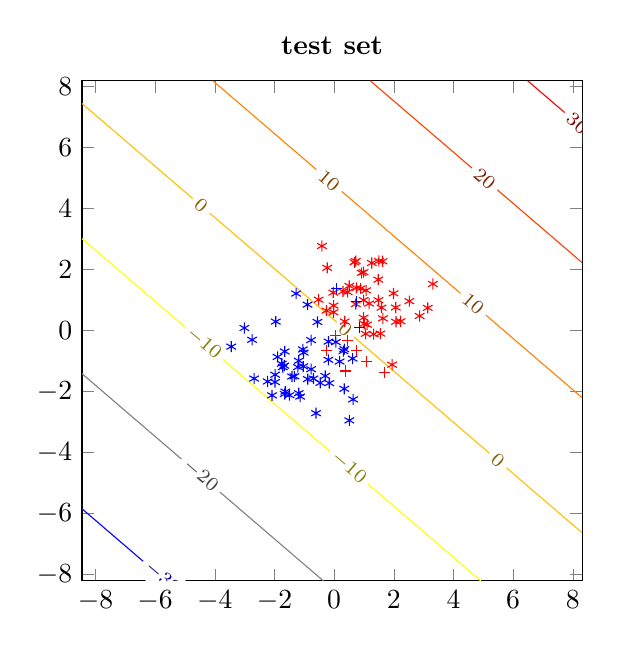
\begin{tikzpicture}

\begin{axis}[%
width=2.5in,
height=2.5in,
at={(0.668056in,0.48125in)},
scale only axis,
xmin=-8.44901775375681,
xmax=8.30928748595239,
ymin=-8.20232071732344,
ymax=8.1831858181971,
title style={font=\bfseries},
title={test set}
]
\addplot[contour prepared, contour prepared format=matlab] table[row sep=crcr] {%
%
-30	13\\
-8.44901775375681	-5.84210674080754\\
-8.13983713383397	-6.10161475123106\\
-8.01931761940529	-6.20277173647289\\
-7.63927642142127	-6.52175594444954\\
-7.58961748505378	-6.56343673213827\\
-7.15991735070226	-6.92410172780362\\
-7.13871570900852	-6.94189713766801\\
-6.73021721635074	-7.28476672346899\\
-6.63815499659581	-7.36203833088649\\
-6.30051708199922	-7.64543171913434\\
-6.13759428418306	-7.78217952410496\\
-5.8708169476477	-8.00609671479971\\
-5.63703357177034	-8.20232071732344\\
-20	36\\
-8.44901775375681	-1.41507109992078\\
-8.37158734590058	-1.48006162582783\\
-8.01931761940529	-1.77573609558611\\
-7.87102663348781	-1.90020281904631\\
-7.58961748505378	-2.13640109125149\\
-7.37046592107511	-2.32034401226478\\
-7.15991735070226	-2.49706608691685\\
-6.86990520866238	-2.74048520548326\\
-6.73021721635074	-2.8577310825822\\
-6.36934449624965	-3.16062639870173\\
-6.30051708199922	-3.21839607824757\\
-5.8708169476477	-3.57906107391293\\
-5.86878378383692	-3.58076759192021\\
-5.44111681329619	-3.93972606957828\\
-5.36822307142419	-4.00090878513868\\
-5.01141667894467	-4.30039106524364\\
-4.86766235901146	-4.42104997835716\\
-4.58171654459315	-4.66105606090901\\
-4.36710164659874	-4.84119117157563\\
-4.15201641024163	-5.02172105657436\\
-3.866540934186	-5.26133236479411\\
-3.72231627589012	-5.38238605223971\\
-3.36598022177329	-5.68147355801259\\
-3.2926161415386	-5.74305104790509\\
-2.86541950936056	-6.10161475123106\\
-2.86291600718708	-6.10371604357045\\
-2.43321587283556	-6.4643810392358\\
-2.36485879694783	-6.52175594444954\\
-2.00351573848404	-6.82504603490116\\
-1.86429808453508	-6.94189713766801\\
-1.57381560413253	-7.18571103056652\\
-1.36373737212237	-7.36203833088649\\
-1.14411546978101	-7.54637602623188\\
-0.863176659709634	-7.78217952410496\\
-0.714415335429489	-7.90704102189723\\
-0.362615947296917	-8.20232071732344\\
-10	59\\
-8.44901775375681	3.011964540966\\
-8.10277684555438	2.72135030635692\\
-8.01931761940529	2.65129954530068\\
-7.6022161331417	2.30120911313845\\
-7.58961748505378	2.29063454963528\\
-7.15991735070226	1.92996955396994\\
-7.10165542072894	1.88106791991997\\
-6.73021721635074	1.56930455830461\\
-6.60109470831619	1.46092672670149\\
-6.30051708199922	1.20863956263922\\
-6.10053399590349	1.04078553348302\\
-5.8708169476477	0.847974566973851\\
-5.59997328349077	0.620644340264543\\
-5.44111681329619	0.487309571308486\\
-5.09941257107805	0.200503147046068\\
-5.01141667894467	0.126644575643124\\
-4.59885185866533	-0.219638046172405\\
-4.58171654459315	-0.234020420022236\\
-4.15201641024163	-0.594685415687577\\
-4.09829114625258	-0.63977923939088\\
-3.72231627589012	-0.955350411352945\\
-3.59773043383986	-1.05992043260936\\
-3.2926161415386	-1.3160154070183\\
-3.09716972142713	-1.48006162582783\\
-2.86291600718708	-1.67668040268366\\
-2.5966090090144	-1.90020281904631\\
-2.43321587283556	-2.03734539834902\\
-2.09604829660166	-2.32034401226478\\
-2.00351573848404	-2.39801039401437\\
-1.59548758418894	-2.74048520548326\\
-1.57381560413253	-2.75867538967974\\
-1.14411546978101	-3.1193403853451\\
-1.09492687177621	-3.16062639870173\\
-0.714415335429489	-3.48000538101046\\
-0.594366159363481	-3.58076759192021\\
-0.284715201077971	-3.84067037667581\\
-0.0938054469507442	-4.00090878513868\\
0.144984933273545	-4.20133537234117\\
0.406755265461971	-4.42104997835716\\
0.574685067625063	-4.56200036800653\\
0.907315977874715	-4.84119117157563\\
1.00438520197658	-4.92266536367189\\
1.40787669028743	-5.26133236479411\\
1.4340853363281	-5.28333035933726\\
1.86378547067962	-5.64399535500261\\
1.90843740270016	-5.68147355801259\\
2.29348560503113	-6.00466035066798\\
2.4089981151129	-6.10161475123106\\
2.72318573938265	-6.36532534633332\\
2.90955882752562	-6.52175594444954\\
3.15288587373417	-6.72599034199867\\
3.41011953993836	-6.94189713766801\\
3.58258600808569	-7.08665533766405\\
3.91068025235107	-7.36203833088649\\
4.01228614243721	-7.44732033332941\\
4.4112409647638	-7.78217952410496\\
4.44198627678873	-7.80798532899478\\
4.87168641114024	-8.1686503246601\\
4.91180167717656	-8.20232071732344\\
0	74\\
-8.44901775375681	7.43900018185279\\
-8.33452705762097	7.34290343176015\\
-8.01931761940529	7.07833518618744\\
-7.83396634520824	6.92276223854167\\
-7.58961748505378	6.71767019052209\\
-7.3334056327955	6.5026210453232\\
-7.15991735070226	6.35700519485672\\
-6.83284492038282	6.08247985210472\\
-6.73021721635074	5.99634019919135\\
-6.33228420797006	5.66233865888625\\
-6.30051708199922	5.635675203526\\
-5.8708169476477	5.27501020786061\\
-5.83172349555736	5.24219746566777\\
-5.44111681329619	4.9143452121953\\
-5.33116278314459	4.8220562724493\\
-5.01141667894467	4.5536802165299\\
-4.8306020707319	4.40191507923082\\
-4.58171654459315	4.19301522086456\\
-4.33004135831917	3.98177388601235\\
-4.15201641024163	3.83235022519919\\
-3.82948064590645	3.56163269279387\\
-3.72231627589012	3.47168522953383\\
-3.32891993349368	3.1414914995754\\
-3.2926161415386	3.11102023386849\\
-2.86291600718708	2.75035523820311\\
-2.82835922108098	2.72135030635692\\
-2.43321587283556	2.38969024253775\\
-2.32779850866825	2.30120911313845\\
-2.00351573848404	2.0290252468724\\
-1.82723779625552	1.88106791991997\\
-1.57381560413253	1.66836025120704\\
-1.32667708384279	1.46092672670149\\
-1.14411546978101	1.30769525554168\\
-0.826116371430058	1.04078553348302\\
-0.714415335429489	0.947030259876319\\
-0.325555659017334	0.620644340264543\\
-0.284715201077971	0.586365264210958\\
0.144984933273545	0.2257002685456\\
0.175005053395395	0.200503147046068\\
0.574685067625063	-0.134964727119756\\
0.675565765808124	-0.219638046172405\\
1.00438520197658	-0.495629722785114\\
1.17612647822085	-0.63977923939088\\
1.4340853363281	-0.856294718450475\\
1.67668719063359	-1.05992043260936\\
1.86378547067962	-1.21695971411582\\
2.17724790304631	-1.48006162582783\\
2.29348560503113	-1.5776247097812\\
2.677808615459	-1.90020281904631\\
2.72318573938265	-1.93828970544658\\
3.15288587373417	-2.29895470111192\\
3.17836932787176	-2.32034401226478\\
3.58258600808569	-2.65961969677725\\
3.67893004028452	-2.74048520548326\\
4.01228614243721	-3.02028469244263\\
4.17949075269723	-3.16062639870173\\
4.44198627678873	-3.38094968810799\\
4.68005146510997	-3.58076759192021\\
4.87168641114024	-3.74161468377334\\
5.1806121775227	-4.00090878513868\\
5.30138654549176	-4.10227967943869\\
5.68117288993546	-4.42104997835716\\
5.73108667984328	-4.46294467510403\\
6.1607868141948	-4.8236096707694\\
6.18173360234818	-4.84119117157563\\
6.59048694854632	-5.18427466643483\\
6.68229431476083	-5.26133236479411\\
7.02018708289783	-5.54493966210017\\
7.18285502717357	-5.68147355801259\\
7.44988721724935	-5.90560465776552\\
7.68341573958635	-6.10161475123106\\
7.87958735160087	-6.26626965343084\\
8.18397645199912	-6.52175594444954\\
8.30928748595239	-6.62693464909617\\
10	54\\
-4.06123085797303	8.1831858181971\\
-3.72231627589012	7.89872087042061\\
-3.56067014556032	7.76304462497863\\
-3.2926161415386	7.53805587475521\\
-3.06010943314753	7.34290343176015\\
-2.86291600718708	7.17739087908991\\
-2.5595487207348	6.92276223854167\\
-2.43321587283556	6.81672588342456\\
-2.0589880083221	6.5026210453232\\
-2.00351573848404	6.45606088775917\\
-1.57381560413253	6.09539589209383\\
-1.55842729590936	6.08247985210472\\
-1.14411546978101	5.73473089642844\\
-1.05786658349666	5.66233865888625\\
-0.714415335429489	5.3740659007631\\
-0.55730587108391	5.24219746566777\\
-0.284715201077971	5.01340090509774\\
-0.056745158671195	4.8220562724493\\
0.144984933273545	4.65273590943237\\
0.443815553741529	4.40191507923082\\
0.574685067625063	4.29207091376701\\
0.944376266154268	3.98177388601235\\
1.00438520197658	3.93140591810165\\
1.4340853363281	3.57074092243632\\
1.44493697856702	3.56163269279387\\
1.86378547067962	3.21007592677094\\
1.94549769097973	3.1414914995754\\
2.29348560503113	2.84941093110558\\
2.44605840339246	2.72135030635692\\
2.72318573938265	2.48874593544022\\
2.94661911580519	2.30120911313845\\
3.15288587373417	2.12808093977487\\
3.44717982821792	1.88106791991997\\
3.58258600808569	1.76741594410951\\
3.94774054063063	1.46092672670149\\
4.01228614243721	1.40675094844413\\
4.44198627678873	1.04608595277879\\
4.44830125304338	1.04078553348302\\
4.87168641114024	0.685420957113439\\
4.94886196545612	0.620644340264543\\
5.30138654549176	0.324755961448065\\
5.44942267786883	0.200503147046068\\
5.73108667984328	-0.0359090342172951\\
5.94998339028156	-0.219638046172405\\
6.1607868141948	-0.396574029882647\\
6.45054410269429	-0.63977923939088\\
6.59048694854632	-0.757239025548003\\
6.951104815107	-1.05992043260936\\
7.02018708289783	-1.11790402121339\\
7.44988721724935	-1.4785690168787\\
7.45166552751978	-1.48006162582783\\
7.87958735160087	-1.83923401254405\\
7.95222623993251	-1.90020281904631\\
8.30928748595239	-2.19989900820942\\
20	32\\
1.21318676650038	8.1831858181971\\
1.4340853363281	7.99777656332306\\
1.71374747891317	7.76304462497863\\
1.86378547067962	7.63711156765774\\
2.21430819132587	7.34290343176015\\
2.29348560503113	7.27644657199235\\
2.71486890373858	6.92276223854167\\
2.72318573938265	6.91578157632698\\
3.15288587373417	6.55511658066165\\
3.21542961615135	6.5026210453232\\
3.58258600808569	6.19445158499629\\
3.71599032856408	6.08247985210472\\
4.01228614243721	5.83378658933093\\
4.2165510409768	5.66233865888625\\
4.44198627678873	5.47312159366556\\
4.71711175338952	5.24219746566777\\
4.87168641114024	5.1124565980002\\
5.21767246580226	4.8220562724493\\
5.30138654549176	4.75179160233485\\
5.71823317821498	4.40191507923082\\
5.73108667984328	4.39112660666948\\
6.1607868141948	4.03046161100413\\
6.21879389062772	3.98177388601235\\
6.59048694854632	3.66979661533877\\
6.71935460304045	3.56163269279387\\
7.02018708289783	3.30913161967342\\
7.21991531545317	3.1414914995754\\
7.44988721724935	2.94846662400805\\
7.72047602786589	2.72135030635692\\
7.87958735160087	2.58780162834267\\
8.22103674027862	2.30120911313845\\
8.30928748595239	2.22713663267733\\
30	9\\
6.48760439097385	8.1831858181971\\
6.59048694854632	8.09683225622554\\
6.98816510338661	7.76304462497863\\
7.02018708289783	7.7361672605602\\
7.44988721724935	7.37550226489482\\
7.48872581579931	7.34290343176015\\
7.87958735160087	7.01483726922946\\
7.98928652821204	6.92276223854167\\
8.30928748595239	6.65417227356411\\
};
\addplot [color=red,only marks,mark=asterisk,mark options={solid},forget plot]
  table[row sep=crcr]{%
1.63527413474712	0.398587873730275\\
};
\addplot [color=red,only marks,mark=asterisk,mark options={solid},forget plot]
  table[row sep=crcr]{%
1.5511847118249	-0.0998404547108134\\
};
\addplot [color=red,only marks,mark=+,mark options={solid},forget plot]
  table[row sep=crcr]{%
1.08599059329372	-1.00456332159079\\
};
\addplot [color=red,only marks,mark=asterisk,mark options={solid},forget plot]
  table[row sep=crcr]{%
0.506912082340303	1.46204801179919\\
};
\addplot [color=red,only marks,mark=asterisk,mark options={solid},forget plot]
  table[row sep=crcr]{%
0.678995307818708	2.23655565160192\\
};
\addplot [color=red,only marks,mark=+,mark options={solid},forget plot]
  table[row sep=crcr]{%
0.368720343274854	-1.32521112888377\\
};
\addplot [color=red,only marks,mark=asterisk,mark options={solid},forget plot]
  table[row sep=crcr]{%
-0.231636533325015	2.05564838790246\\
};
\addplot [color=red,only marks,mark=asterisk,mark options={solid},forget plot]
  table[row sep=crcr]{%
0.886776010630975	1.37922362268503\\
};
\addplot [color=red,only marks,mark=asterisk,mark options={solid},forget plot]
  table[row sep=crcr]{%
1.94419972674731	-1.12042668822421\\
};
\addplot [color=red,only marks,mark=asterisk,mark options={solid},forget plot]
  table[row sep=crcr]{%
0.355321084458063	0.295698271566391\\
};
\addplot [color=red,only marks,mark=asterisk,mark options={solid},forget plot]
  table[row sep=crcr]{%
-0.0181372163990707	0.817918131588615\\
};
\addplot [color=red,only marks,mark=asterisk,mark options={solid},forget plot]
  table[row sep=crcr]{%
2.52101323900559	0.961561236113288\\
};
\addplot [color=red,only marks,mark=asterisk,mark options={solid},forget plot]
  table[row sep=crcr]{%
2.22744798900972	0.303795199967111\\
};
\addplot [color=red,only marks,mark=asterisk,mark options={solid},forget plot]
  table[row sep=crcr]{%
1.00752448652301	0.217106955621713\\
};
\addplot [color=red,only marks,mark=asterisk,mark options={solid},forget plot]
  table[row sep=crcr]{%
1.58693855921443	0.748792625431118\\
};
\addplot [color=red,only marks,mark=asterisk,mark options={solid},forget plot]
  table[row sep=crcr]{%
1.4801358228426	1.66815503443364\\
};
\addplot [color=red,only marks,mark=asterisk,mark options={solid},forget plot]
  table[row sep=crcr]{%
0.921678803726588	1.8891726184126\\
};
\addplot [color=red,only marks,mark=asterisk,mark options={solid},forget plot]
  table[row sep=crcr]{%
3.30928748595239	1.5246386797711\\
};
\addplot [color=red,only marks,mark=asterisk,mark options={solid},forget plot]
  table[row sep=crcr]{%
0.988212676048693	1.91314081776137\\
};
\addplot [color=red,only marks,mark=asterisk,mark options={solid},forget plot]
  table[row sep=crcr]{%
1.0559406788884	-0.107069894826007\\
};
\addplot [color=red,only marks,mark=asterisk,mark options={solid},forget plot]
  table[row sep=crcr]{%
1.48549770731281	0.994994926244469\\
};
\addplot [color=red,only marks,mark=asterisk,mark options={solid},forget plot]
  table[row sep=crcr]{%
0.723782140645241	2.27645247367439\\
};
\addplot [color=red,only marks,mark=asterisk,mark options={solid},forget plot]
  table[row sep=crcr]{%
2.86340061318454	0.477440698363601\\
};
\addplot [color=red,only marks,mark=asterisk,mark options={solid},forget plot]
  table[row sep=crcr]{%
1.10342444693731	0.19235086910282\\
};
\addplot [color=red,only marks,mark=+,mark options={solid},forget plot]
  table[row sep=crcr]{%
1.68043858374895	-1.36458984794158\\
};
\addplot [color=red,only marks,mark=asterisk,mark options={solid},forget plot]
  table[row sep=crcr]{%
1.99011487204949	1.21889912088118\\
};
\addplot [color=red,only marks,mark=asterisk,mark options={solid},forget plot]
  table[row sep=crcr]{%
1.2616624601614	2.21344449497535\\
};
\addplot [color=red,only marks,mark=asterisk,mark options={solid},forget plot]
  table[row sep=crcr]{%
0.725333013543219	0.866865549186471\\
};
\addplot [color=red,only marks,mark=+,mark options={solid},forget plot]
  table[row sep=crcr]{%
-0.270500203708377	-0.663606452829772\\
};
\addplot [color=red,only marks,mark=asterisk,mark options={solid},forget plot]
  table[row sep=crcr]{%
0.296445738463245	1.2808804885233\\
};
\addplot [color=red,only marks,mark=+,mark options={solid},forget plot]
  table[row sep=crcr]{%
0.458790670083806	-0.333530729736393\\
};
\addplot [color=red,only marks,mark=asterisk,mark options={solid},forget plot]
  table[row sep=crcr]{%
2.07268626789014	0.287914547505644\\
};
\addplot [color=red,only marks,mark=asterisk,mark options={solid},forget plot]
  table[row sep=crcr]{%
0.988714438769314	0.999182970804304\\
};
\addplot [color=red,only marks,mark=asterisk,mark options={solid},forget plot]
  table[row sep=crcr]{%
0.750563715304566	1.39657531871165\\
};
\addplot [color=red,only marks,mark=+,mark options={solid},forget plot]
  table[row sep=crcr]{%
0.735986645077757	-0.664010876930589\\
};
\addplot [color=red,only marks,mark=asterisk,mark options={solid},forget plot]
  table[row sep=crcr]{%
-0.028975099543801	1.24309470022456\\
};
\addplot [color=red,only marks,mark=asterisk,mark options={solid},forget plot]
  table[row sep=crcr]{%
-0.256590107833817	0.652816810266474\\
};
\addplot [color=red,only marks,mark=+,mark options={solid},forget plot]
  table[row sep=crcr]{%
0.0586278065716714	-0.174560281302444\\
};
\addplot [color=red,only marks,mark=asterisk,mark options={solid},forget plot]
  table[row sep=crcr]{%
-0.021141686935775	0.598333265403212\\
};
\addplot [color=red,only marks,mark=asterisk,mark options={solid},forget plot]
  table[row sep=crcr]{%
1.17366566856231	0.883881506649489\\
};
\addplot [color=red,only marks,mark=asterisk,mark options={solid},forget plot]
  table[row sep=crcr]{%
2.06411914898635	0.75461370324833\\
};
\addplot [color=red,only marks,mark=asterisk,mark options={solid},forget plot]
  table[row sep=crcr]{%
-0.517539131089556	1.00973415912595\\
};
\addplot [color=red,only marks,mark=asterisk,mark options={solid},forget plot]
  table[row sep=crcr]{%
1.07137286485595	1.31653581376851\\
};
\addplot [color=red,only marks,mark=asterisk,mark options={solid},forget plot]
  table[row sep=crcr]{%
1.49982566779648	2.27808414671411\\
};
\addplot [color=red,only marks,mark=asterisk,mark options={solid},forget plot]
  table[row sep=crcr]{%
0.452183853078842	1.26080839887907\\
};
\addplot [color=red,only marks,mark=asterisk,mark options={solid},forget plot]
  table[row sep=crcr]{%
0.986823328126488	0.419735997858047\\
};
\addplot [color=red,only marks,mark=asterisk,mark options={solid},forget plot]
  table[row sep=crcr]{%
3.13630842280531	0.742382884346519\\
};
\addplot [color=red,only marks,mark=asterisk,mark options={solid},forget plot]
  table[row sep=crcr]{%
-0.409528489369198	2.77010089285161\\
};
\addplot [color=red,only marks,mark=asterisk,mark options={solid},forget plot]
  table[row sep=crcr]{%
1.32554598476071	-0.119039575381312\\
};
\addplot [color=red,only marks,mark=asterisk,mark options={solid},forget plot]
  table[row sep=crcr]{%
1.62035013944552	2.26978184718977\\
};
\addplot [color=blue,only marks,mark=asterisk,mark options={solid},forget plot]
  table[row sep=crcr]{%
-1.89604250642191	-0.864824555241563\\
};
\addplot [color=blue,only marks,mark=asterisk,mark options={solid},forget plot]
  table[row sep=crcr]{%
-1.13904001004044	-2.16339529383727\\
};
\addplot [color=blue,only marks,mark=asterisk,mark options={solid},forget plot]
  table[row sep=crcr]{%
0.183719539936857	-1.01542966178332\\
};
\addplot [color=blue,only marks,mark=asterisk,mark options={solid},forget plot]
  table[row sep=crcr]{%
-0.463781305281383	-1.71642862372586\\
};
\addplot [color=blue,only marks,mark=asterisk,mark options={solid},forget plot]
  table[row sep=crcr]{%
-1.65555938950391	-0.685637236689252\\
};
\addplot [color=blue,only marks,mark=asterisk,mark options={solid},forget plot]
  table[row sep=crcr]{%
-0.893185924065412	0.848216218018969\\
};
\addplot [color=blue,only marks,mark=asterisk,mark options={solid},forget plot]
  table[row sep=crcr]{%
-1.27510567543881	1.21255407898968\\
};
\addplot [color=blue,only marks,mark=asterisk,mark options={solid},forget plot]
  table[row sep=crcr]{%
0.508525756096147	-2.94507859991933\\
};
\addplot [color=blue,only marks,mark=asterisk,mark options={solid},forget plot]
  table[row sep=crcr]{%
-2.68054277752265	-1.57353413410588\\
};
\addplot [color=blue,only marks,mark=asterisk,mark options={solid},forget plot]
  table[row sep=crcr]{%
-1.18581652736766	-0.991065884323432\\
};
\addplot [color=blue,only marks,mark=asterisk,mark options={solid},forget plot]
  table[row sep=crcr]{%
-0.163050109162705	-1.7222706724333\\
};
\addplot [color=blue,only marks,mark=asterisk,mark options={solid},forget plot]
  table[row sep=crcr]{%
-1.72149047716441	-1.20118099951714\\
};
\addplot [color=blue,only marks,mark=asterisk,mark options={solid},forget plot]
  table[row sep=crcr]{%
-1.02046416109514	-0.721110000087549\\
};
\addplot [color=blue,only marks,mark=asterisk,mark options={solid},forget plot]
  table[row sep=crcr]{%
0.05829481445	-0.37832671759759\\
};
\addplot [color=blue,only marks,mark=asterisk,mark options={solid},forget plot]
  table[row sep=crcr]{%
-2.75061528848538	-0.302652448516563\\
};
\addplot [color=blue,only marks,mark=asterisk,mark options={solid},forget plot]
  table[row sep=crcr]{%
-0.188514136683007	-0.363655052395867\\
};
\addplot [color=blue,only marks,mark=asterisk,mark options={solid},forget plot]
  table[row sep=crcr]{%
0.310080341410262	-0.672902484081802\\
};
\addplot [color=blue,only marks,mark=asterisk,mark options={solid},forget plot]
  table[row sep=crcr]{%
-1.67299316385471	-1.14932749947673\\
};
\addplot [color=blue,only marks,mark=asterisk,mark options={solid},forget plot]
  table[row sep=crcr]{%
-3.44901775375681	-0.526714387756446\\
};
\addplot [color=blue,only marks,mark=asterisk,mark options={solid},forget plot]
  table[row sep=crcr]{%
-0.883054343206712	-1.5911038386322\\
};
\addplot [color=blue,only marks,mark=asterisk,mark options={solid},forget plot]
  table[row sep=crcr]{%
-1.65470767508278	-2.08066185121169\\
};
\addplot [color=blue,only marks,mark=asterisk,mark options={solid},forget plot]
  table[row sep=crcr]{%
-1.04773086529791	-0.620655462711205\\
};
\addplot [color=blue,only marks,mark=asterisk,mark options={solid},forget plot]
  table[row sep=crcr]{%
-1.33036104579866	-1.49989825118473\\
};
\addplot [color=blue,only marks,mark=asterisk,mark options={solid},forget plot]
  table[row sep=crcr]{%
-1.03597860795301	-1.17476033119672\\
};
\addplot [color=blue,only marks,mark=asterisk,mark options={solid},forget plot]
  table[row sep=crcr]{%
-1.95726507882166	0.292547900132268\\
};
\addplot [color=blue,only marks,mark=asterisk,mark options={solid},forget plot]
  table[row sep=crcr]{%
-0.559090357152978	0.280940942744541\\
};
\addplot [color=blue,only marks,mark=asterisk,mark options={solid},forget plot]
  table[row sep=crcr]{%
-1.49772980521188	-2.11871663760432\\
};
\addplot [color=blue,only marks,mark=asterisk,mark options={solid},forget plot]
  table[row sep=crcr]{%
-0.192350380560649	-0.958800421361755\\
};
\addplot [color=blue,only marks,mark=asterisk,mark options={solid},forget plot]
  table[row sep=crcr]{%
-1.7562086055467	-1.08912914780643\\
};
\addplot [color=blue,only marks,mark=asterisk,mark options={solid},forget plot]
  table[row sep=crcr]{%
-3.00885032178915	0.0839180379588267\\
};
\addplot [color=blue,only marks,mark=asterisk,mark options={solid},forget plot]
  table[row sep=crcr]{%
-1.98119056314417	-1.6884886374647\\
};
\addplot [color=blue,only marks,mark=asterisk,mark options={solid},forget plot]
  table[row sep=crcr]{%
0.339479481807799	-1.90924316031601\\
};
\addplot [color=blue,only marks,mark=asterisk,mark options={solid},forget plot]
  table[row sep=crcr]{%
-1.4128577286188	-1.50616318564854\\
};
\addplot [color=blue,only marks,mark=asterisk,mark options={solid},forget plot]
  table[row sep=crcr]{%
0.619747799125372	-0.9190992887935\\
};
\addplot [color=blue,only marks,mark=asterisk,mark options={solid},forget plot]
  table[row sep=crcr]{%
-2.08105649017694	-2.1245178115942\\
};
\addplot [color=blue,only marks,mark=+,mark options={solid},forget plot]
  table[row sep=crcr]{%
0.735676342606296	0.937458596526754\\
};
\addplot [color=blue,only marks,mark=asterisk,mark options={solid},forget plot]
  table[row sep=crcr]{%
0.635068218520641	-2.25594016677432\\
};
\addplot [color=blue,only marks,mark=asterisk,mark options={solid},forget plot]
  table[row sep=crcr]{%
-1.2135375062087	-1.19893204828268\\
};
\addplot [color=blue,only marks,mark=asterisk,mark options={solid},forget plot]
  table[row sep=crcr]{%
-0.692500822520151	-1.57232545648506\\
};
\addplot [color=blue,only marks,mark=asterisk,mark options={solid},forget plot]
  table[row sep=crcr]{%
-1.97764836704206	-1.44680940665695\\
};
\addplot [color=blue,only marks,mark=+,mark options={solid},forget plot]
  table[row sep=crcr]{%
0.0820919008951635	1.37264794938999\\
};
\addplot [color=blue,only marks,mark=asterisk,mark options={solid},forget plot]
  table[row sep=crcr]{%
-0.770711663895569	-1.26662313612389\\
};
\addplot [color=blue,only marks,mark=asterisk,mark options={solid},forget plot]
  table[row sep=crcr]{%
-0.2983278230806	-1.48759049128981\\
};
\addplot [color=blue,only marks,mark=+,mark options={solid},forget plot]
  table[row sep=crcr]{%
0.862479725319099	0.106851110391344\\
};
\addplot [color=blue,only marks,mark=asterisk,mark options={solid},forget plot]
  table[row sep=crcr]{%
-2.22756572221585	-1.66988511005649\\
};
\addplot [color=blue,only marks,mark=asterisk,mark options={solid},forget plot]
  table[row sep=crcr]{%
0.340929452331313	-0.611916683758858\\
};
\addplot [color=blue,only marks,mark=asterisk,mark options={solid},forget plot]
  table[row sep=crcr]{%
-0.606941071223	-2.70733357783774\\
};
\addplot [color=blue,only marks,mark=asterisk,mark options={solid},forget plot]
  table[row sep=crcr]{%
-0.772141355295662	-0.314367142237049\\
};
\addplot [color=blue,only marks,mark=asterisk,mark options={solid},forget plot]
  table[row sep=crcr]{%
-1.63679011291329	-2.00260555423381\\
};
\addplot [color=blue,only marks,mark=asterisk,mark options={solid},forget plot]
  table[row sep=crcr]{%
-1.18562067291102	-2.05403271420003\\
};
\end{axis}
\end{tikzpicture}%
\end{document}
% This file was created by matlab2tikz.
% Minimal pgfplots version: 1.3
%
%The latest updates can be retrieved from
%  http://www.mathworks.com/matlabcentral/fileexchange/22022-matlab2tikz
%where you can also make suggestions and rate matlab2tikz.
%
\documentclass[tikz]{standalone}
\usepackage{pgfplots}
\usepackage{grffile}
\pgfplotsset{compat=newest}
\usetikzlibrary{plotmarks}
\usepackage{amsmath}

\begin{document}
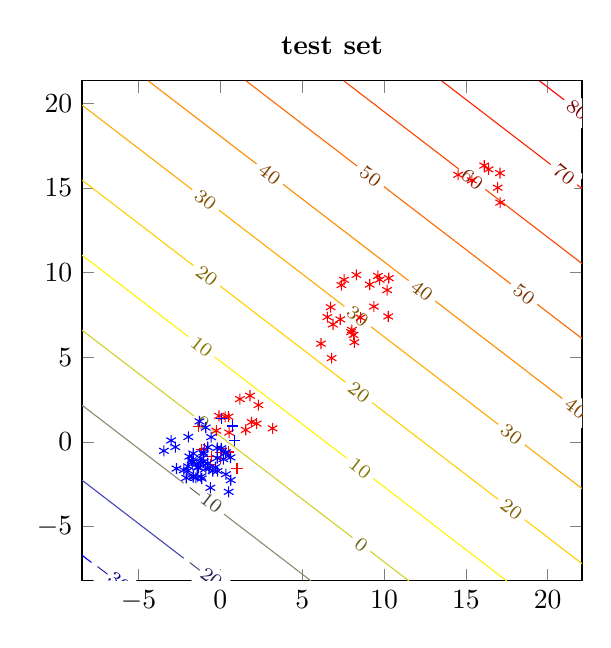
\begin{tikzpicture}

\begin{axis}[%
width=2.5in,
height=2.5in,
at={(0.668056in,0.48125in)},
scale only axis,
xmin=-8.44901775375681,
xmax=22.0950037387875,
ymin=-8.20232071732344,
ymax=21.3148090433951,
title style={font=\bfseries},
title={test set}
]
\addplot[contour prepared, contour prepared format=matlab] table[row sep=crcr] {%
%
-30	5\\
-8.44901775375681	-6.69077815523522\\
-7.66583771548645	-7.27132991834563\\
-7.43091636529865	-7.44547123627937\\
-6.88265767721608	-7.85188168145606\\
-6.40990593488808	-8.20232071732344\\
-20	19\\
-8.44901775375681	-2.261872924265\\
-7.66583771548645	-2.84242468737542\\
-7.58226594421673	-2.90437435001499\\
-6.88265767721608	-3.42297645048583\\
-6.56125551380612	-3.66122383105906\\
-6.09947763894571	-4.00352821359625\\
-5.54024508339555	-4.41807331210312\\
-5.31629760067535	-4.58407997670668\\
-4.53311756240498	-5.1646317398171\\
-4.51923465298496	-5.17492279314718\\
-3.74993752413461	-5.74518350292752\\
-3.49822422257436	-5.93177227419125\\
-2.96675748586425	-6.32573526603793\\
-2.47721379216376	-6.68862175523531\\
-2.18357744759388	-6.90628702914834\\
-1.45620336175319	-7.44547123627937\\
-1.40039740932351	-7.48683879225879\\
-0.617217371053146	-8.06739055536921\\
-0.435192931342599	-8.20232071732344\\
-10	32\\
-8.44901775375681	2.16703230670524\\
-7.73361552313474	1.63672253624939\\
-7.66583771548645	1.58648054359484\\
-6.88265767721608	1.0059287804844\\
-6.71260509272417	0.879873055205328\\
-6.09947763894571	0.42537701737397\\
-5.69159466231359	0.123023574161264\\
-5.31629760067535	-0.155174745736444\\
-4.670584231903	-0.633825906882799\\
-4.53311756240498	-0.735726508846872\\
-3.74993752413461	-1.3162782719573\\
-3.64957380149242	-1.39067538792686\\
-2.96675748586425	-1.89683003506772\\
-2.62856337108183	-2.14752486897093\\
-2.18357744759388	-2.47738179817813\\
-1.60755294067124	-2.90437435001499\\
-1.40039740932351	-3.05793356128855\\
-0.617217371053146	-3.63848532439898\\
-0.586542510260652	-3.66122383105906\\
0.165962667217221	-4.2190370875094\\
0.434467920149933	-4.41807331210312\\
0.949142705487589	-4.79958885061983\\
1.45547835056052	-5.17492279314718\\
1.73232274375795	-5.38014061373025\\
2.47648878097114	-5.93177227419125\\
2.51550278202832	-5.96069237684064\\
3.29868282029869	-6.54124413995108\\
3.4974992113817	-6.68862175523531\\
4.08186285856906	-7.12179590306151\\
4.5185096417923	-7.44547123627937\\
4.86504289683942	-7.70234766617192\\
5.5395200722029	-8.20232071732344\\
0	46\\
-8.44901775375681	6.59593753767546\\
-7.88496510205284	6.17781942251378\\
-7.66583771548645	6.01538577456503\\
-6.88265767721608	5.43483401145461\\
-6.86395467164225	5.42096994146971\\
-6.09947763894571	4.8542822483442\\
-5.84294424123164	4.66412046042565\\
-5.31629760067535	4.27373048523377\\
-4.82193381082106	3.90727097938158\\
-4.53311756240498	3.69317872212335\\
-3.80092338041047	3.15042149833752\\
-3.74993752413461	3.11262695901293\\
-2.96675748586425	2.53207519590251\\
-2.77991294999988	2.39357201729346\\
-2.18357744759388	1.95152343279209\\
-1.75890251958929	1.63672253624939\\
-1.40039740932351	1.37097166968167\\
-0.737892089178704	0.879873055205328\\
-0.617217371053146	0.790419906571245\\
0.165962667217221	0.209868143460825\\
0.283118341231886	0.123023574161264\\
0.949142705487589	-0.370683619649598\\
1.30412877164247	-0.633825906882799\\
1.73232274375795	-0.951235382760018\\
2.32513920205306	-1.39067538792686\\
2.51550278202832	-1.53178714587044\\
3.29868282029869	-2.11233890898086\\
3.34614963246365	-2.14752486897093\\
4.08186285856906	-2.69289067209127\\
4.36716006287425	-2.90437435001499\\
4.86504289683942	-3.27344243520169\\
5.38817049328483	-3.66122383105906\\
5.64822293510979	-3.85399419831213\\
6.40918092369539	-4.41807331210312\\
6.43140297338016	-4.43454596142256\\
7.21458301165052	-5.01509772453297\\
7.430191354106	-5.17492279314718\\
7.99776304992089	-5.59564948764338\\
8.4512017845166	-5.93177227419125\\
8.78094308819126	-6.17620125075381\\
9.4722122149272	-6.68862175523531\\
9.56412312646162	-6.75675301386422\\
10.347303164732	-7.33730477697461\\
10.4932226453378	-7.44547123627937\\
11.1304832030024	-7.91785654008508\\
11.5142330757484	-8.20232071732344\\
10	60\\
-8.44901775375681	11.0248427686457\\
-8.03631468097088	10.7189163087782\\
-7.66583771548645	10.4442910055353\\
-7.01530425056029	9.9620668277341\\
-6.88265767721608	9.86373924242484\\
-6.09947763894571	9.28318747931442\\
-5.9942938201497	9.20521734669003\\
-5.31629760067535	8.70263571620399\\
-4.97328338973912	8.44836786564597\\
-4.53311756240498	8.12208395309356\\
-3.95227295932853	7.6915183846019\\
-3.74993752413461	7.54153218998315\\
-2.96675748586425	6.96098042687272\\
-2.93126252891795	6.93466890355784\\
-2.18357744759388	6.38042866376231\\
-1.91025209850735	6.17781942251378\\
-1.40039740932351	5.79987690065189\\
-0.889241668096753	5.42096994146971\\
-0.617217371053146	5.21932513754146\\
0.131768762313821	4.66412046042565\\
0.165962667217221	4.63877337443104\\
0.949142705487589	4.05822161132062\\
1.15277919272442	3.90727097938158\\
1.73232274375795	3.47766984821021\\
2.17378962313501	3.15042149833752\\
2.51550278202832	2.89711808509978\\
3.19480005354559	2.39357201729346\\
3.29868282029869	2.31656632198935\\
4.08186285856906	1.73601455887895\\
4.2158104839562	1.63672253624939\\
4.86504289683942	1.15546279576853\\
5.23682091436678	0.879873055205328\\
5.64822293510979	0.574911032658096\\
6.25783134477737	0.123023574161264\\
6.43140297338016	-0.00564073045231372\\
7.21458301165052	-0.586192493562759\\
7.27884177518793	-0.633825906882799\\
7.99776304992089	-1.16674425667315\\
8.29985220559854	-1.39067538792686\\
8.78094308819126	-1.74729601978358\\
9.32086263600915	-2.14752486897093\\
9.56412312646162	-2.32784778289399\\
10.3418730664197	-2.90437435001499\\
10.347303164732	-2.90839954600444\\
11.1304832030024	-3.48895130911487\\
11.3628834968303	-3.66122383105906\\
11.9136632412727	-4.06950307222525\\
12.3838939272409	-4.41807331210312\\
12.6968432795431	-4.65005483533568\\
13.4049043576515	-5.17492279314718\\
13.4800233178135	-5.23060659844608\\
14.2632033560838	-5.81115836155652\\
14.4259147880621	-5.93177227419125\\
15.0463833943542	-6.39171012466694\\
15.4469252184727	-6.68862175523531\\
15.8295634326246	-6.97226188777737\\
16.4679356488833	-7.44547123627937\\
16.6127434708949	-7.55281365088777\\
17.3959235091653	-8.13336541399824\\
17.4889460792938	-8.20232071732344\\
20	70\\
-8.44901775375681	15.4537479996159\\
-8.18766425988888	15.2600131950425\\
-7.66583771548645	14.8731962365055\\
-7.16665382947838	14.5031637139985\\
-6.88265767721608	14.292644473395\\
-6.14564339906775	13.7463142329544\\
-6.09947763894571	13.7120927102846\\
-5.31629760067535	13.1315409471742\\
-5.12463296865717	12.9894647519104\\
-4.53311756240498	12.5509891840638\\
-4.10362253824658	12.2326152708663\\
-3.74993752413461	11.9704374209534\\
-3.08261210783597	11.4757657898222\\
-2.96675748586425	11.389885657843\\
-2.18357744759388	10.8093338947325\\
-2.06160167742539	10.7189163087782\\
-1.40039740932351	10.2287821316221\\
-1.04059124701481	9.9620668277341\\
-0.617217371053146	9.6482303685117\\
-0.0195808166042212	9.20521734669003\\
0.165962667217221	9.06767860540127\\
0.949142705487589	8.48712684229085\\
1.00142961380637	8.44836786564597\\
1.73232274375795	7.90657507918044\\
2.02244004421697	7.6915183846019\\
2.51550278202832	7.32602331607001\\
3.04345047462755	6.93466890355784\\
3.29868282029869	6.7454715529596\\
4.06446090503816	6.17781942251378\\
4.08186285856906	6.16491978984918\\
4.86504289683942	5.58436802673875\\
5.08547133544872	5.42096994146971\\
5.64822293510979	5.00381626362833\\
6.10648176585931	4.66412046042565\\
6.43140297338016	4.4232645005179\\
7.12749219626989	3.90727097938158\\
7.21458301165052	3.84271273740748\\
7.99776304992089	3.26216097429704\\
8.14850262668046	3.15042149833752\\
8.78094308819126	2.68160921118662\\
9.16951305709105	2.39357201729346\\
9.56412312646162	2.1010574480762\\
10.1905234875017	1.63672253624939\\
10.347303164732	1.52050568496579\\
11.1304832030024	0.939953921855371\\
11.2115339179123	0.879873055205328\\
11.9136632412727	0.359402158744985\\
12.2325443483229	0.123023574161264\\
12.6968432795431	-0.221149604365461\\
13.2535547787334	-0.633825906882799\\
13.4800233178135	-0.80170136747589\\
14.2632033560838	-1.38225313058633\\
14.274565209144	-1.39067538792686\\
15.0463833943542	-1.96280489369671\\
15.2955756395546	-2.14752486897093\\
15.8295634326246	-2.54335665680713\\
16.3165860699652	-2.90437435001499\\
16.6127434708949	-3.12390841991758\\
17.3375965003759	-3.66122383105906\\
17.3959235091653	-3.70446018302793\\
18.1791035474357	-4.28501194613839\\
18.3586069307864	-4.41807331210312\\
18.962283585706	-4.86556370924883\\
19.3796173611969	-5.17492279314718\\
19.7454636239764	-5.44611547235932\\
20.4006277916075	-5.93177227419125\\
20.5286436622468	-6.0266672354697\\
21.3118237005171	-6.60721899858007\\
21.4216382220182	-6.68862175523531\\
22.0950037387875	-7.18777076169053\\
30	70\\
-8.44901775375681	19.8826532305861\\
-8.33901383880697	19.8011100813069\\
-7.66583771548645	19.3021014674757\\
-7.31800340839641	19.0442606002629\\
-6.88265767721608	18.7215497043653\\
-6.29699297798578	18.2874111192188\\
-6.09947763894571	18.1409979412549\\
-5.31629760067535	17.5604461781444\\
-5.27598254757525	17.5305616381747\\
-4.53311756240498	16.979894415034\\
-4.25497211716461	16.7737121571307\\
-3.74993752413461	16.3993426519236\\
-3.23396168675404	16.0168626760866\\
-2.96675748586425	15.8187908888132\\
-2.21295125634341	15.2600131950425\\
-2.18357744759388	15.2382391257028\\
-1.40039740932351	14.6576873625924\\
-1.19194082593284	14.5031637139985\\
-0.617217371053146	14.0771355994819\\
-0.170930395522275	13.7463142329544\\
0.165962667217221	13.4965838363715\\
0.850080034888325	12.9894647519104\\
0.949142705487589	12.9160320732611\\
1.73232274375795	12.3354803101507\\
1.8710904652989	12.2326152708663\\
2.51550278202832	11.7549285470403\\
2.8921008957095	11.4757657898222\\
3.29868282029869	11.1743767839298\\
3.91311132612007	10.7189163087782\\
4.08186285856906	10.5938250208194\\
4.86504289683942	10.013273257709\\
4.93412175653067	9.9620668277341\\
5.64822293510979	9.43272149459855\\
5.95513218694125	9.20521734669003\\
6.43140297338016	8.85216973148812\\
6.97614261735185	8.44836786564597\\
7.21458301165052	8.27161796837771\\
7.99715304776245	7.6915183846019\\
7.99776304992089	7.6910662052673\\
8.78094308819126	7.11051444215684\\
9.018163478173	6.93466890355784\\
9.56412312646162	6.52996267904644\\
10.0391739085836	6.17781942251378\\
10.347303164732	5.94941091593603\\
11.0601843389943	5.42096994146971\\
11.1304832030024	5.36885915282564\\
11.9136632412727	4.78830738971518\\
12.0811947694048	4.66412046042565\\
12.6968432795431	4.20775562660479\\
13.1022051998154	3.90727097938158\\
13.4800233178135	3.62720386349436\\
14.123215630226	3.15042149833752\\
14.2632033560838	3.04665210038392\\
15.0463833943542	2.46610033727351\\
15.1442260606366	2.39357201729346\\
15.8295634326246	1.88554857416309\\
16.1652364910472	1.63672253624939\\
16.6127434708949	1.30499681105268\\
17.1862469214577	0.879873055205328\\
17.3959235091653	0.724445047942197\\
18.1791035474357	0.143893284831826\\
18.2072573518683	0.123023574161264\\
18.962283585706	-0.436658478278624\\
19.2282677822789	-0.633825906882799\\
19.7454636239764	-1.017210241389\\
20.2492782126895	-1.39067538792686\\
20.5286436622468	-1.59776200449946\\
21.2702886431001	-2.14752486897093\\
21.3118237005171	-2.17831376760984\\
22.0950037387875	-2.75886553072035\\
40	60\\
-4.40632169608275	21.3148090433951\\
-3.74993752413461	20.8282478828938\\
-3.38531126567218	20.557959562351\\
-2.96675748586425	20.2476961197834\\
-2.36430083526152	19.8011100813069\\
-2.18357744759388	19.667144356673\\
-1.40039740932351	19.0865925935625\\
-1.34329040485094	19.0442606002629\\
-0.617217371053146	18.5060408304521\\
-0.322279974440309	18.2874111192188\\
0.165962667217221	17.9254890673417\\
0.698730455970253	17.5305616381747\\
0.949142705487589	17.3449373042313\\
1.71974088638085	16.7737121571307\\
1.73232274375795	16.7643855411209\\
2.51550278202832	16.1838337780104\\
2.74075131679143	16.0168626760866\\
3.29868282029869	15.6032820149001\\
3.76176174720205	15.2600131950425\\
4.08186285856906	15.0227302517896\\
4.78277217761265	14.5031637139985\\
4.86504289683942	14.4421784886792\\
5.64822293510979	13.8616267255688\\
5.8037826080232	13.7463142329544\\
6.43140297338016	13.2810749624584\\
6.82479303843381	12.9894647519104\\
7.21458301165052	12.7005231993479\\
7.84580346884439	12.2326152708663\\
7.99776304992089	12.1199714362375\\
8.78094308819126	11.5394196731271\\
8.866813899255	11.4757657898222\\
9.56412312646162	10.9588679100167\\
9.88782432966554	10.7189163087782\\
10.347303164732	10.3783161469062\\
10.9088347600761	9.9620668277341\\
11.1304832030024	9.7977643837958\\
11.9136632412727	9.2172126206854\\
11.9298451904867	9.20521734669003\\
12.6968432795431	8.636660857575\\
12.9508556208973	8.44836786564597\\
13.4800233178135	8.05610909446457\\
13.9718660513079	7.6915183846019\\
14.2632033560838	7.47555733135413\\
14.9928764817186	6.93466890355784\\
15.0463833943542	6.89500556824376\\
15.8295634326246	6.31445380513327\\
16.013886912129	6.17781942251378\\
16.6127434708949	5.73390204202288\\
17.0348973425397	5.42096994146971\\
17.3959235091653	5.15335027891248\\
18.0559077729503	4.66412046042565\\
18.1791035474357	4.57279851580203\\
18.962283585706	3.99224675269163\\
19.0769182033609	3.90727097938158\\
19.7454636239764	3.41169498958116\\
20.0979286337714	3.15042149833752\\
20.5286436622468	2.8311432264708\\
21.118939064182	2.39357201729346\\
21.3118237005171	2.25059146336035\\
22.0950037387875	1.67003970024992\\
50	48\\
1.56839130746274	21.3148090433951\\
1.73232274375795	21.1932907720911\\
2.51550278202832	20.6127390089807\\
2.58940173787338	20.557959562351\\
3.29868282029869	20.0321872458703\\
3.61041216828396	19.8011100813069\\
4.08186285856906	19.4516354827598\\
4.63142259869459	19.0442606002629\\
4.86504289683942	18.8710837196494\\
5.64822293510979	18.290531956539\\
5.65243302910516	18.2874111192188\\
6.43140297338016	17.7099801934286\\
6.67344345951572	17.5305616381747\\
7.21458301165052	17.1294284303181\\
7.69445388992631	16.7737121571307\\
7.99776304992089	16.5488766672077\\
8.71546432033694	16.0168626760866\\
8.78094308819126	15.9683249040973\\
9.56412312646162	15.3877731409869\\
9.73647475074751	15.2600131950425\\
10.347303164732	14.8072213778765\\
10.7574851811581	14.5031637139985\\
11.1304832030024	14.2266696147661\\
11.7784956115687	13.7463142329544\\
11.9136632412727	13.6461178516556\\
12.6968432795431	13.0655660885452\\
12.7995060419793	12.9894647519104\\
13.4800233178135	12.4850143254348\\
13.8205164723899	12.2326152708663\\
14.2632033560838	11.9044625623244\\
14.8415269028004	11.4757657898222\\
15.0463833943542	11.3239107992139\\
15.8295634326246	10.7433590361035\\
15.8625373332111	10.7189163087782\\
16.6127434708949	10.1628072729931\\
16.8835477636217	9.9620668277341\\
17.3959235091653	9.58225550988269\\
17.9045581940322	9.20521734669003\\
18.1791035474357	9.00170374677227\\
18.9255686244428	8.44836786564597\\
18.962283585706	8.42115198366183\\
19.7454636239764	7.8406002205514\\
19.9465790548534	7.6915183846019\\
20.5286436622468	7.26004845744096\\
20.967589485264	6.93466890355784\\
21.3118237005171	6.67949669433061\\
21.9885999156746	6.17781942251378\\
22.0950037387875	6.09894493122016\\
60	34\\
7.54310431100827	21.3148090433951\\
7.99776304992089	20.977781898178\\
8.56411474141886	20.557959562351\\
8.78094308819126	20.3972301350675\\
9.56412312646162	19.8166783719571\\
9.58512517182947	19.8011100813069\\
10.347303164732	19.2361266088467\\
10.6061356022401	19.0442606002629\\
11.1304832030024	18.6555748457363\\
11.6271460326506	18.2874111192188\\
11.9136632412727	18.0750230826258\\
12.6481564630612	17.5305616381747\\
12.6968432795431	17.4944713195154\\
13.4800233178135	16.913919556405\\
13.6691668934718	16.7737121571307\\
14.2632033560838	16.3333677932946\\
14.6901773238824	16.0168626760866\\
15.0463833943542	15.7528160301842\\
15.711187754293	15.2600131950425\\
15.8295634326246	15.1722642670738\\
16.6127434708949	14.5917125039633\\
16.7321981847035	14.5031637139985\\
17.3959235091653	14.0111607408529\\
17.7532086151142	13.7463142329544\\
18.1791035474357	13.4306089777425\\
18.7742190455248	12.9894647519104\\
18.962283585706	12.8500572146321\\
19.7454636239764	12.2695054515217\\
19.7952294759354	12.2326152708663\\
20.5286436622468	11.6889536884112\\
20.8162399063459	11.4757657898222\\
21.3118237005171	11.1084019253008\\
21.8372503367565	10.7189163087782\\
22.0950037387875	10.5278501621903\\
70	20\\
13.5178173145538	21.3148090433951\\
14.2632033560838	20.7622730242648\\
14.5388277449643	20.557959562351\\
15.0463833943542	20.1817212611544\\
15.559838175375	19.8011100813069\\
15.8295634326246	19.601169498044\\
16.5808486057855	19.0442606002629\\
16.6127434708949	19.0206177349336\\
17.3959235091653	18.4400659718231\\
17.6018590361961	18.2874111192188\\
18.1791035474357	17.8595142087127\\
18.6228694666067	17.5305616381747\\
18.962283585706	17.2789624456023\\
19.6438798970172	16.7737121571307\\
19.7454636239764	16.6984106824918\\
20.5286436622468	16.1178589193815\\
20.6648903274279	16.0168626760866\\
21.3118237005171	15.537307156271\\
21.6859007578385	15.2600131950425\\
22.0950037387875	14.9567553931606\\
80	7\\
19.4925303180992	21.3148090433951\\
19.7454636239764	21.1273159134621\\
20.5135407485099	20.557959562351\\
20.5286436622468	20.5467641503517\\
21.3118237005171	19.9662123872413\\
21.5345511789204	19.8011100813069\\
22.0950037387875	19.3856606241308\\
};
\addplot [color=red,only marks,mark=asterisk,mark options={solid},forget plot]
  table[row sep=crcr]{%
-0.2463365280849	0.663024145855908\\
};
\addplot [color=red,only marks,mark=+,mark options={solid},forget plot]
  table[row sep=crcr]{%
0.0558011901764726	-0.367873566740638\\
};
\addplot [color=red,only marks,mark=asterisk,mark options={solid},forget plot]
  table[row sep=crcr]{%
9.62323385113849	9.79904861814778\\
};
\addplot [color=red,only marks,mark=asterisk,mark options={solid},forget plot]
  table[row sep=crcr]{%
-0.0793302230234205	1.53515226612215\\
};
\addplot [color=red,only marks,mark=asterisk,mark options={solid},forget plot]
  table[row sep=crcr]{%
0.535397954249106	0.552883517423822\\
};
\addplot [color=red,only marks,mark=asterisk,mark options={solid},forget plot]
  table[row sep=crcr]{%
9.38033725171391	7.99088447565921\\
};
\addplot [color=red,only marks,mark=+,mark options={solid},forget plot]
  table[row sep=crcr]{%
0.0112448963841337	-0.64514581569117\\
};
\addplot [color=red,only marks,mark=asterisk,mark options={solid},forget plot]
  table[row sep=crcr]{%
9.73095733842945	9.5778573463308\\
};
\addplot [color=red,only marks,mark=asterisk,mark options={solid},forget plot]
  table[row sep=crcr]{%
3.19083807424337	0.797542885226056\\
};
\addplot [color=red,only marks,mark=asterisk,mark options={solid},forget plot]
  table[row sep=crcr]{%
2.21932067266762	1.07809837564446\\
};
\addplot [color=red,only marks,mark=asterisk,mark options={solid},forget plot]
  table[row sep=crcr]{%
2.32729236140865	2.17463914282092\\
};
\addplot [color=red,only marks,mark=+,mark options={solid},forget plot]
  table[row sep=crcr]{%
-0.606482859277266	-1.34736267385024\\
};
\addplot [color=red,only marks,mark=asterisk,mark options={solid},forget plot]
  table[row sep=crcr]{%
0.497769664182782	1.48849047090348\\
};
\addplot [color=red,only marks,mark=+,mark options={solid},forget plot]
  table[row sep=crcr]{%
-1.31943699810954	0.931217514995436\\
};
\addplot [color=red,only marks,mark=+,mark options={solid},forget plot]
  table[row sep=crcr]{%
0.485295555916544	-0.595490902619476\\
};
\addplot [color=red,only marks,mark=+,mark options={solid},forget plot]
  table[row sep=crcr]{%
-0.546475894767623	-0.846758163883059\\
};
\addplot [color=red,only marks,mark=asterisk,mark options={solid},forget plot]
  table[row sep=crcr]{%
1.19490959580312	2.52874301096222\\
};
\addplot [color=red,only marks,mark=+,mark options={solid},forget plot]
  table[row sep=crcr]{%
-0.947146064738541	-0.374429195029166\\
};
\addplot [color=red,only marks,mark=+,mark options={solid},forget plot]
  table[row sep=crcr]{%
0.0214661388790944	-1.00394446674772\\
};
\addplot [color=red,only marks,mark=+,mark options={solid},forget plot]
  table[row sep=crcr]{%
-1.16781936472664	-0.460605179506151\\
};
\addplot [color=red,only marks,mark=asterisk,mark options={solid},forget plot]
  table[row sep=crcr]{%
1.90435159451633	1.16765053634998\\
};
\addplot [color=red,only marks,mark=asterisk,mark options={solid},forget plot]
  table[row sep=crcr]{%
0.289502034538413	1.47891705768128\\
};
\addplot [color=red,only marks,mark=asterisk,mark options={solid},forget plot]
  table[row sep=crcr]{%
1.81329142231856	2.7257905482933\\
};
\addplot [color=red,only marks,mark=+,mark options={solid},forget plot]
  table[row sep=crcr]{%
1.01841178862471	-1.58040249930316\\
};
\addplot [color=red,only marks,mark=asterisk,mark options={solid},forget plot]
  table[row sep=crcr]{%
1.55324256851535	0.707893884632476\\
};
\addplot [color=red,only marks,mark=asterisk,mark options={solid},forget plot]
  table[row sep=crcr]{%
8.1902449362512	5.88379124221439\\
};
\addplot [color=red,only marks,mark=asterisk,mark options={solid},forget plot]
  table[row sep=crcr]{%
10.2902497549325	9.66860050568204\\
};
\addplot [color=red,only marks,mark=asterisk,mark options={solid},forget plot]
  table[row sep=crcr]{%
15.3645347745207	15.4404266978038\\
};
\addplot [color=red,only marks,mark=asterisk,mark options={solid},forget plot]
  table[row sep=crcr]{%
16.1184448370541	16.3148090433951\\
};
\addplot [color=red,only marks,mark=asterisk,mark options={solid},forget plot]
  table[row sep=crcr]{%
16.9408899407278	15.0079082644562\\
};
\addplot [color=red,only marks,mark=asterisk,mark options={solid},forget plot]
  table[row sep=crcr]{%
8.03783419871876	6.61020045152317\\
};
\addplot [color=red,only marks,mark=asterisk,mark options={solid},forget plot]
  table[row sep=crcr]{%
6.53502663282888	7.37096058384895\\
};
\addplot [color=red,only marks,mark=asterisk,mark options={solid},forget plot]
  table[row sep=crcr]{%
10.1891642016521	8.96236672340668\\
};
\addplot [color=red,only marks,mark=asterisk,mark options={solid},forget plot]
  table[row sep=crcr]{%
7.39591443799884	9.25730423467749\\
};
\addplot [color=red,only marks,mark=asterisk,mark options={solid},forget plot]
  table[row sep=crcr]{%
8.30822429829771	9.85799667282826\\
};
\addplot [color=red,only marks,mark=asterisk,mark options={solid},forget plot]
  table[row sep=crcr]{%
8.13802801285837	6.31586141486366\\
};
\addplot [color=red,only marks,mark=asterisk,mark options={solid},forget plot]
  table[row sep=crcr]{%
6.14580262553102	5.79868518466096\\
};
\addplot [color=red,only marks,mark=asterisk,mark options={solid},forget plot]
  table[row sep=crcr]{%
7.32736756408083	7.23405701284718\\
};
\addplot [color=red,only marks,mark=asterisk,mark options={solid},forget plot]
  table[row sep=crcr]{%
14.5248654941447	15.765995952344\\
};
\addplot [color=red,only marks,mark=asterisk,mark options={solid},forget plot]
  table[row sep=crcr]{%
7.98633739100202	6.48136493365525\\
};
\addplot [color=red,only marks,mark=asterisk,mark options={solid},forget plot]
  table[row sep=crcr]{%
17.0822949531553	15.8685002970547\\
};
\addplot [color=red,only marks,mark=asterisk,mark options={solid},forget plot]
  table[row sep=crcr]{%
8.56743518847178	7.3344156217619\\
};
\addplot [color=red,only marks,mark=asterisk,mark options={solid},forget plot]
  table[row sep=crcr]{%
6.88013057194261	6.93470598515841\\
};
\addplot [color=red,only marks,mark=asterisk,mark options={solid},forget plot]
  table[row sep=crcr]{%
6.79630952043264	4.94567531944339\\
};
\addplot [color=red,only marks,mark=asterisk,mark options={solid},forget plot]
  table[row sep=crcr]{%
7.55903556809898	9.57114762365818\\
};
\addplot [color=red,only marks,mark=asterisk,mark options={solid},forget plot]
  table[row sep=crcr]{%
16.389880489687	16.0879871065798\\
};
\addplot [color=red,only marks,mark=asterisk,mark options={solid},forget plot]
  table[row sep=crcr]{%
9.12533230647483	9.28767642035855\\
};
\addplot [color=red,only marks,mark=asterisk,mark options={solid},forget plot]
  table[row sep=crcr]{%
10.2540014216025	7.40627042355252\\
};
\addplot [color=red,only marks,mark=asterisk,mark options={solid},forget plot]
  table[row sep=crcr]{%
17.0950037387875	14.126009742359\\
};
\addplot [color=red,only marks,mark=asterisk,mark options={solid},forget plot]
  table[row sep=crcr]{%
6.73889837693838	7.95346544550482\\
};
\addplot [color=blue,only marks,mark=asterisk,mark options={solid},forget plot]
  table[row sep=crcr]{%
-1.89604250642191	-0.864824555241563\\
};
\addplot [color=blue,only marks,mark=asterisk,mark options={solid},forget plot]
  table[row sep=crcr]{%
-1.13904001004044	-2.16339529383727\\
};
\addplot [color=blue,only marks,mark=asterisk,mark options={solid},forget plot]
  table[row sep=crcr]{%
0.183719539936857	-1.01542966178332\\
};
\addplot [color=blue,only marks,mark=asterisk,mark options={solid},forget plot]
  table[row sep=crcr]{%
-0.463781305281383	-1.71642862372586\\
};
\addplot [color=blue,only marks,mark=asterisk,mark options={solid},forget plot]
  table[row sep=crcr]{%
-1.65555938950391	-0.685637236689252\\
};
\addplot [color=blue,only marks,mark=asterisk,mark options={solid},forget plot]
  table[row sep=crcr]{%
-0.893185924065412	0.848216218018969\\
};
\addplot [color=blue,only marks,mark=asterisk,mark options={solid},forget plot]
  table[row sep=crcr]{%
-1.27510567543881	1.21255407898968\\
};
\addplot [color=blue,only marks,mark=asterisk,mark options={solid},forget plot]
  table[row sep=crcr]{%
0.508525756096147	-2.94507859991933\\
};
\addplot [color=blue,only marks,mark=asterisk,mark options={solid},forget plot]
  table[row sep=crcr]{%
-2.68054277752265	-1.57353413410588\\
};
\addplot [color=blue,only marks,mark=asterisk,mark options={solid},forget plot]
  table[row sep=crcr]{%
-1.18581652736766	-0.991065884323432\\
};
\addplot [color=blue,only marks,mark=asterisk,mark options={solid},forget plot]
  table[row sep=crcr]{%
-0.163050109162705	-1.7222706724333\\
};
\addplot [color=blue,only marks,mark=asterisk,mark options={solid},forget plot]
  table[row sep=crcr]{%
-1.72149047716441	-1.20118099951714\\
};
\addplot [color=blue,only marks,mark=asterisk,mark options={solid},forget plot]
  table[row sep=crcr]{%
-1.02046416109514	-0.721110000087549\\
};
\addplot [color=blue,only marks,mark=asterisk,mark options={solid},forget plot]
  table[row sep=crcr]{%
0.05829481445	-0.37832671759759\\
};
\addplot [color=blue,only marks,mark=asterisk,mark options={solid},forget plot]
  table[row sep=crcr]{%
-2.75061528848538	-0.302652448516563\\
};
\addplot [color=blue,only marks,mark=asterisk,mark options={solid},forget plot]
  table[row sep=crcr]{%
-0.188514136683007	-0.363655052395867\\
};
\addplot [color=blue,only marks,mark=asterisk,mark options={solid},forget plot]
  table[row sep=crcr]{%
0.310080341410262	-0.672902484081802\\
};
\addplot [color=blue,only marks,mark=asterisk,mark options={solid},forget plot]
  table[row sep=crcr]{%
-1.67299316385471	-1.14932749947673\\
};
\addplot [color=blue,only marks,mark=asterisk,mark options={solid},forget plot]
  table[row sep=crcr]{%
-3.44901775375681	-0.526714387756446\\
};
\addplot [color=blue,only marks,mark=asterisk,mark options={solid},forget plot]
  table[row sep=crcr]{%
-0.883054343206712	-1.5911038386322\\
};
\addplot [color=blue,only marks,mark=asterisk,mark options={solid},forget plot]
  table[row sep=crcr]{%
-1.65470767508278	-2.08066185121169\\
};
\addplot [color=blue,only marks,mark=asterisk,mark options={solid},forget plot]
  table[row sep=crcr]{%
-1.04773086529791	-0.620655462711205\\
};
\addplot [color=blue,only marks,mark=asterisk,mark options={solid},forget plot]
  table[row sep=crcr]{%
-1.33036104579866	-1.49989825118473\\
};
\addplot [color=blue,only marks,mark=asterisk,mark options={solid},forget plot]
  table[row sep=crcr]{%
-1.03597860795301	-1.17476033119672\\
};
\addplot [color=blue,only marks,mark=asterisk,mark options={solid},forget plot]
  table[row sep=crcr]{%
-1.95726507882166	0.292547900132268\\
};
\addplot [color=blue,only marks,mark=asterisk,mark options={solid},forget plot]
  table[row sep=crcr]{%
-0.559090357152978	0.280940942744541\\
};
\addplot [color=blue,only marks,mark=asterisk,mark options={solid},forget plot]
  table[row sep=crcr]{%
-1.49772980521188	-2.11871663760432\\
};
\addplot [color=blue,only marks,mark=asterisk,mark options={solid},forget plot]
  table[row sep=crcr]{%
-0.192350380560649	-0.958800421361755\\
};
\addplot [color=blue,only marks,mark=asterisk,mark options={solid},forget plot]
  table[row sep=crcr]{%
-1.7562086055467	-1.08912914780643\\
};
\addplot [color=blue,only marks,mark=asterisk,mark options={solid},forget plot]
  table[row sep=crcr]{%
-3.00885032178915	0.0839180379588267\\
};
\addplot [color=blue,only marks,mark=asterisk,mark options={solid},forget plot]
  table[row sep=crcr]{%
-1.98119056314417	-1.6884886374647\\
};
\addplot [color=blue,only marks,mark=asterisk,mark options={solid},forget plot]
  table[row sep=crcr]{%
0.339479481807799	-1.90924316031601\\
};
\addplot [color=blue,only marks,mark=asterisk,mark options={solid},forget plot]
  table[row sep=crcr]{%
-1.4128577286188	-1.50616318564854\\
};
\addplot [color=blue,only marks,mark=asterisk,mark options={solid},forget plot]
  table[row sep=crcr]{%
0.619747799125372	-0.9190992887935\\
};
\addplot [color=blue,only marks,mark=asterisk,mark options={solid},forget plot]
  table[row sep=crcr]{%
-2.08105649017694	-2.1245178115942\\
};
\addplot [color=blue,only marks,mark=+,mark options={solid},forget plot]
  table[row sep=crcr]{%
0.735676342606296	0.937458596526754\\
};
\addplot [color=blue,only marks,mark=asterisk,mark options={solid},forget plot]
  table[row sep=crcr]{%
0.635068218520641	-2.25594016677432\\
};
\addplot [color=blue,only marks,mark=asterisk,mark options={solid},forget plot]
  table[row sep=crcr]{%
-1.2135375062087	-1.19893204828268\\
};
\addplot [color=blue,only marks,mark=asterisk,mark options={solid},forget plot]
  table[row sep=crcr]{%
-0.692500822520151	-1.57232545648506\\
};
\addplot [color=blue,only marks,mark=asterisk,mark options={solid},forget plot]
  table[row sep=crcr]{%
-1.97764836704206	-1.44680940665695\\
};
\addplot [color=blue,only marks,mark=+,mark options={solid},forget plot]
  table[row sep=crcr]{%
0.0820919008951635	1.37264794938999\\
};
\addplot [color=blue,only marks,mark=asterisk,mark options={solid},forget plot]
  table[row sep=crcr]{%
-0.770711663895569	-1.26662313612389\\
};
\addplot [color=blue,only marks,mark=asterisk,mark options={solid},forget plot]
  table[row sep=crcr]{%
-0.2983278230806	-1.48759049128981\\
};
\addplot [color=blue,only marks,mark=+,mark options={solid},forget plot]
  table[row sep=crcr]{%
0.862479725319099	0.106851110391344\\
};
\addplot [color=blue,only marks,mark=asterisk,mark options={solid},forget plot]
  table[row sep=crcr]{%
-2.22756572221585	-1.66988511005649\\
};
\addplot [color=blue,only marks,mark=asterisk,mark options={solid},forget plot]
  table[row sep=crcr]{%
0.340929452331313	-0.611916683758858\\
};
\addplot [color=blue,only marks,mark=asterisk,mark options={solid},forget plot]
  table[row sep=crcr]{%
-0.606941071223	-2.70733357783774\\
};
\addplot [color=blue,only marks,mark=asterisk,mark options={solid},forget plot]
  table[row sep=crcr]{%
-0.772141355295662	-0.314367142237049\\
};
\addplot [color=blue,only marks,mark=asterisk,mark options={solid},forget plot]
  table[row sep=crcr]{%
-1.63679011291329	-2.00260555423381\\
};
\addplot [color=blue,only marks,mark=asterisk,mark options={solid},forget plot]
  table[row sep=crcr]{%
-1.18562067291102	-2.05403271420003\\
};
\end{axis}
\end{tikzpicture}%
\end{document}
\caption{Geometrical construction of a linear classification line using average values.}
\label{fig:initGaussSvm}
\end{figure}

\section{Vapnik Support Vector machines}
At the hart of vapnik's theory is the optimal hyperplane algorithm. In the linear the hyperplane condition is given as\footnote{Support-Vector Networks
CORINNA CORTES VLADIMIR VAPNIK,Machine Leaming, 20, (1995) page 291 or Least Squares Support Vector Machines, Suykens et al., page 31.}
\begin{equation}
y_k [\mathbf{w}^T \mathbf{x}_k + b] \geq 1, \;\; k = 1,\dots,N
\end{equation}
With $x_k$ being the input data points and $y_k$ the desired output. Training the machine means finding the high dimensional hyperplane normal vector $w$ and the bias scalar $b$. Normal means here that the dot product with any vector lying in the plane must be zero. Technically a plane is defined by $\mathbf{w}^T(\mathbf{x} - \mathbf{p}) = 0$ but its only interesting here to evaluate the classifier so $b = \mathbf{p}^T \mathbf{w}$ can be used instead and the displacement within the feature space remains unknown.
The next step is to formulate the optimization problem
\begin{equation}
\min_{w,b} \frac{1}{2} \mathbf{w}^T \mathbf{w} \;\text{ such that }\; y_k [\mathbf{w}^T \mathbf{x}_k + b] \geq 1.
\end{equation}
Formulating the Lagrange dual, and taking the gradient of $\mathcal{L}(\mathbf{w},b;\alpha)$ with respect to $(\mathbf{w},b)$ leads to a problem in $\alpha$. The lagrange multipliers are called $\alpha$, but in this context they will be called support vectors of the solution. From an optimization point of view, the support vectors are Lagrange multipliers with active set indices. A problem reformulation as
\begin{equation}
y_k [\mathbf{w}^T \phi(\mathbf{x}_k) + b] \geq 1
\end{equation}
allows for different kernel options. The classifier is given by
\begin{equation}
y(\mathbf{x}) = \text{sign}(\sum^N_{k=1} \alpha_k y_k K(\mathbf{x},\mathbf{x}_k) + b).
\end{equation}
The following three kernels will be considered here\footnote{Suykens, Data Mining and Neural Networks, Cursustekst page 140.}
\begin{align}
K(\mathbf{x},\mathbf{x}_k)  &= \mathbf{x}_k^T \mathbf{x} &\text{  (linear SVM)}, \\
K(\mathbf{x}, \mathbf{x}_k) &= \exp (-\| \mathbf{x} - \mathbf{x}_k \|^2_2 / \sigma^2) &\text{  (RBF Kernel)}.
\end{align}
If the problem is not separable, it means that classification cannot be done without error. In the underlying optimization problem slack variables have to be included in the formulation. 



\begin{figure}
\centering
\includegraphics[width=0.33\linewidth]{../src/figure/svmjsLinSep}
\includegraphics[width=0.33\linewidth]{../src/figure/svmjsLinRBF}
\caption{Support vector machine classification of an almost linearly separable problem using a linear and an radial basis function kernel}
\label{fig:svmjsLinRBF}
\end{figure}


\section{Least Squares Support Vector machines}